\documentclass{article}

\usepackage[utf8]{inputenc}
\usepackage[T1]{fontenc}
\usepackage{geometry}
\geometry{margin=1in}
\usepackage{hyperref}
\usepackage{url}
\usepackage{booktabs}
\usepackage{amsfonts}
\usepackage{amsmath}
\usepackage{amssymb}
\usepackage{microtype}
\usepackage{graphicx}
\usepackage{multirow}
\usepackage{enumitem}
\usepackage{fancyhdr}

\graphicspath{{media/}}

\providecommand{\keywords}[1]{\par\noindent\textbf{Keywords: }#1}
\newcommand{\achf}{\textsc{ACHF}}
\newcommand{\ama}{\textsc{AMA}}
\newcommand{\achfbox}[2]{%
\fbox{\begin{minipage}{#1}\centering #2\end{minipage}}%
}

\pagestyle{fancy}
\thispagestyle{empty}
\rhead{\textit{}}
\fancyhead[LO]{ACHF: Adaptive Cache-aware Hyper-Connections}

\title{
\achf{}: Adaptive Cache-aware Hyper-Connections\\
A Guarded Runtime Design and Single-CPU Case Study
}

\author{
Stephen F. Zhuang\\
\texttt{info@zayoka.com}
}

\begin{document}

\maketitle

\begin{abstract}
Neural inference cost depends on memory layout, sparse-dispatch overhead, reuse,
and device behavior as well as arithmetic. \achf{} (Adaptive Cache-aware
Hyper-Connections) separates three decisions that are often conflated: whether
a semantic candidate is accurate enough to replace a stable reference,
which equivalent physical realization should execute an admitted candidate,
and whether an exact output may be reused. During training, a constrained
connection coefficient and a candidate-specific gate define a soft
reference--candidate blend. After calibration, frozen inference uses a hard
reference/candidate decision followed by \ama{}, a guarded selector over
prepared-dense, sparse, and ordinary-dense realizations. Exact memoization is
orthogonal to both decisions.

We evaluate a Rust CPU implementation in three independent operating-system
processes with five paired trials per process and Student-$t$ intervals over
process means ($N=3$). On a same-run exploratory admission frontier, the
$51.001\%$ candidate was the only tested point admitted in all 15 trials; its
output-relative error was $4.084\%$ (95\% CI $[3.926,4.242]\%$). The measured
runtime instantiation kept its training gate inactive. Relative to the dense
reference, it reduced end-to-end throughput by $16.62\%$
($[-18.05,-15.19]\%$), added $14.225$ s of training, and produced unresolved
reward and loss differences. Its materialized inference state was $4.235\times$
the reference-parameter bytes. At the admitted point, a prepared-dense
candidate was faster than sparse traversal. Sparse execution had nominal
paired 95\% intervals below both alternatives only at $0.95$ and $0.99$
sparsity in the exploratory crossover grid.
Guarded \ama{} had a lower mean oracle gap than Plain EMA at seven of eight
independently warmed operating points; paired intervals were below zero at six
and unresolved at two. These results support guarded admission and conditional
selector performance on this steady-state grid, not universal quality,
efficiency, active training-gate, memoization-speedup, or regime-transition
claims.
\end{abstract}

\keywords{
Hyper-Connections,
Runtime-adaptive Inference,
Sparse Neural Execution,
Guarded Adaptation,
Constrained Connection Mapping,
Neural Runtime Systems
}

\section{Introduction}

Residual connections are one of the most reliable architectural devices in
modern neural networks because they preserve an identity path while allowing
learnable transformations to refine the representation
\cite{he2016deep,he2016identity}. Hyper-Connection style architectures
generalize this idea by widening or diversifying the connection topology
\cite{hyperconnections2024,mhc2025}. This can improve expressivity, but it also
changes the stability and memory-access profile of the network.

Deployment exposes a different pressure. A layer can look cheap on paper and
still run poorly in the program that executes it. Sparse traversal may reduce
multiply-adds while losing locality. A dense cached view of a pruned operator
may beat a sparse traversal when shapes repeat. A connection that helps during
training may also need a different realization during inference. These effects
show up in policy models, transformers, feed-forward networks, and other
components whose latency is governed as much by memory movement as by
arithmetic.

\achf{} addresses this gap by treating a hyper-connection as both a
representational object and an execution object. It distinguishes a semantic
candidate $c$ from a physical realization $p\in\mathcal{P}(c)$. The former may
change the layer function and must pass a quality-admission predicate; the
latter is one of several numerically equivalent ways to execute an already
admitted candidate. Exact input--output memoization is a third, orthogonal
layer. \ama{} controls physical realization selection from measured runtime
state. Talos-XII is the case-study runtime, not part of either definition.

The central claim is deliberately narrow. \achf{} is not primarily a pruning
recipe, an MoE router, or an early-exit policy. It is a connection-level
adaptation method: a layer preserves a stable reference computation while
exposing one or more semantic candidates whose training participation is
controlled by optimization and discrepancy signals. After calibration, a hard
quality boundary chooses the reference or an admitted candidate. \ama{} then
selects an execution realization only when its validity, measured cost,
stale-latency state, and switching controls permit it. Gradient alignment and
optimizer-state drift are recorded as training diagnostics; they are not
execution guards in the evaluated implementation. This separates \emph{what
function a layer represents}, \emph{how that function executes}, and \emph{when
an exact result can be reused}.

The main contributions are:

\begin{itemize}[leftmargin=*]
\item \textbf{Three-layer formulation.} A reference/candidate quality layer,
an execution layer indexed by $p\in\mathcal{P}(c)$, and exact memoized reuse,
with separate training-soft and frozen-hard equations.
\item \textbf{Constrained and guarded execution formulation.} A dedicated
connection map that enters the training mixer, plus proposed \ama{} validity,
economic, stale-measurement, and switching controls for realizations of an
admitted candidate. The evaluated case study instantiates only the guarded
ranking and probing subset.
\item \textbf{Auditable case study.} A ten-experiment, three-process CPU study
covering admission, invariants, fixed-path crossover, and independently warmed
selector operating points while retaining regressions and unresolved outcomes.
\end{itemize}

\subsection{Claim Boundary}

The method claim and the empirical claim are kept separate. The method claim is
that Equations~\eqref{eq:achf-tuple}--\eqref{eq:achf-path-selector} define a
connection-level mechanism combining a stable reference, semantic candidates,
a constrained training mixer, hard post-calibration admission, physical
realization selection, and exact reuse. \ama{} is the separate guarded procedure in
Equations~\eqref{eq:ama-state}--\eqref{eq:ama-objective}; it can be applied to
ACHF but is not defined by ACHF. The implementation claim is narrower:
Talos-XII instantiates one ACHF--\ama{} configuration in a compact Rust runtime.

No universal reward, accuracy, latency, or convergence improvement is claimed
here. The measurements in Section~\ref{sec:experiments} reject a general
efficiency claim for the current compact CPU implementation: the measured ACHF
runtime instantiation with an inactive training gate is
slower than the dense reference and takes longer to train, while reward and
loss differences are unresolved. The supported empirical claims are narrower:
the configured admission rule excludes candidates outside its boundary, the
fastest execution realization changes with dimension and sparsity, and Guarded
\ama{} has lower mean oracle gaps than Plain EMA at seven of eight steady-state
points, with paired intervals below zero at six. Comparisons with dynamic depth, MoE routing,
additional tasks, and additional hardware remain outside the measured scope.

Figure~\ref{fig:achf-overview} summarizes the proposed mechanism. The figure is
intended to describe the general ACHF layer, not the full Talos-XII runtime.

\begin{figure}[t]
\centering
\small
\setlength{\fboxsep}{5pt}
\begin{minipage}{\linewidth}
\centering
\textbf{ACHF layer at runtime step \(t\)}\\[0.8em]
\begin{tabular*}{\linewidth}{@{\extracolsep{\fill}}c c c c c}
\achfbox{0.14\linewidth}{Input\\\(h_l\)}
&
\(\longrightarrow\)
&
\achfbox{0.28\linewidth}{Quality layer\\Reference \(F_{\theta_l}\)\\semantic candidate \(C_{\phi_{l,c}}\)}
&
\(\longrightarrow\)
&
\achfbox{0.24\linewidth}{Training output\\soft blend}
\end{tabular*}
\\[1.0em]
\begin{tabular*}{\linewidth}{@{\extracolsep{\fill}}c c c c c}
\achfbox{0.18\linewidth}{Connection map\\\(\bar R_l=\mathsf{Scale}(R_l)\)\\candidate coefficient}
&
\(\longrightarrow\)
&
\achfbox{0.27\linewidth}{Post-calibration\\quality admission \(A_{c,l}\)\\hard reference/candidate}
&
\(\longrightarrow\)
&
\achfbox{0.24\linewidth}{Execution selector\\\(p\in\mathcal{P}_l(c)\)\\prepared / sparse / dense}
\end{tabular*}
\\[1.0em]
\begin{tabular*}{\linewidth}{@{\extracolsep{\fill}}c c c c c}
\achfbox{0.22\linewidth}{Training statistics\\gradient proxy \(q_{l,t}\)\\candidate discrepancy \(d_{k,l,t}\)}
&
\(\longrightarrow\)
&
\achfbox{0.18\linewidth}{Adaptive gate\\\(g_{k,l,t}\in[g_{\min,t},1]\)}
&
\(\longrightarrow\)
&
\achfbox{0.30\linewidth}{Reference--candidate blend\\\((1-a_{c,l,t})F_{\theta_l}(h_l)+a_{c,l,t}C_{\phi_{l,c}}(h_l)\)}
\end{tabular*}
\\[1.0em]
\begin{tabular*}{\linewidth}{@{\extracolsep{\fill}}c c c c c}
\achfbox{0.24\linewidth}{Runtime measurements\\latency EMA, sparsity, warmness, stale age}
&
\(\longrightarrow\)
&
\achfbox{0.18\linewidth}{State\\\(\mathcal{S}_t\)}
&
\(\longrightarrow\)
&
\achfbox{0.20\linewidth}{Exact reuse layer\\state epoch + full input\\hit or execute \(p^*\)}
\end{tabular*}
\end{minipage}
\caption{
Overview of an \achf{} layer. During training, optimization statistics and
reference--candidate discrepancy drive a soft gate, while a constrained
connection coefficient enters the same mixer. Frozen inference makes a hard
quality decision before \ama{} chooses an equivalent physical realization.
Exact memoized reuse has a state-qualified key and is independent of both
decisions.
}
\label{fig:achf-overview}
\end{figure}

\section{Background and Motivation}

\subsection{Residual and Hyper-Connection Stability}

A standard residual block can be written as
\begin{equation}
x_{l+1}=x_l+F_l(x_l).
\label{eq:residual}
\end{equation}
The identity term helps preserve signal and gradient flow across depth.
Hyper-Connection variants extend this idea by introducing learnable connection
maps around the residual branch. A broad form is
\begin{equation}
x_{l+1}=H_{\mathrm{res}}x_l+
H_{\mathrm{post}}^\top F_l(H_{\mathrm{pre}}x_l).
\label{eq:hyperconnection}
\end{equation}

The additional maps increase topological flexibility, but unconstrained
connection matrices can amplify, cancel, or poorly condition signals.
Manifold-constrained Hyper-Connections use constraints such as
Sinkhorn-Knopp projection to make the connection maps better behaved
\cite{sinkhorn1967concerning,mhc2025}. The lesson adopted by \achf{} is not
that every runtime must reproduce the full hyper-connection topology. Instead,
connection operators that alter identity or feed-forward paths need explicit
constraints and observable diagnostics.

\subsection{Runtime Bottlenecks in Neural Inference}

Inference workloads frequently operate under irregular batch sizes, changing
sequence lengths, repeated activation patterns, and device-specific memory
behavior. In this regime, theoretical FLOP reduction can be a poor proxy for
end-to-end latency. Sparse traversal may save arithmetic while losing cache
locality. A cached dense layout of a pruned matrix may be faster than a sparse
kernel for repeated input shapes. Therefore \achf{} makes inference path
selection a runtime decision rather than a static assumption.

\section{Related Work and Positioning}
\label{sec:related}

\subsection{Hyper-Connections and Manifold-constrained Hyper-Connections}

Hyper-Connections generalize residual connectivity by introducing learnable
connection maps around the transformation path \cite{hyperconnections2024}.
mHC extends this direction by constraining those connection maps on a manifold,
for example through Sinkhorn-style normalization, so that the added connection
freedom remains better conditioned \cite{mhc2025}. Their central object is the
\emph{connection topology}: how information is mixed, transported, and
stabilized across the network.

\achf{} borrows the idea that connection behavior needs to be explicit and
constrained, but it changes the object under study. The \achf{} layer in
Equation~\eqref{eq:achf-tuple} keeps a reference operator, admits semantic
candidates such as pruned, low-rank, or quantized operators, and then chooses
among function-equivalent physical realizations of an admitted candidate. The
question is therefore not only whether the connection map is expressive or
well conditioned, but whether a candidate is accurate enough and how that same
candidate should execute.

This distinction matters for both claims and experiments. A successful mHC
result would show that manifold-constrained connection maps improve
optimization or representation. A successful \achf{} result has to show something
different: that preserving a reference path while selecting among candidate
realizations improves a measured runtime or quality--latency tradeoff after
selector overhead is counted. Talos-XII also does not implement the full
dynamic $H_{\mathrm{pre}}$, $H_{\mathrm{post}}$, and $H_{\mathrm{res}}$ stack
from mHC. It uses constrained projection and dense--candidate execution as a
practical \achf{} instance.

\ama{} is even further separated from Hyper-Connections. It is not a
connection-topology proposal. It is a guarded control algorithm for physical
realizations of an already admitted computation. A Hyper-Connection, an
\achf{} layer, a quantized layer, or a device dispatcher could all be controlled
by \ama{}, but \ama{} itself neither defines the connection map nor decides
semantic candidate quality.

\subsection{Dynamic Inference and Conditional Computation}

Dynamic neural networks adapt computation at inference time rather than using a
single fixed graph for every input. Surveys commonly organize this area around
instance-wise, spatial-wise, and temporal-wise adaptivity
\cite{han2021dynamic}. Early-exit models such as BranchyNet attach auxiliary
classifiers to intermediate layers and stop computation when the prediction is
confident enough \cite{teerapittayanon2016branchynet}. Adaptive Computation
Time learns how many recurrent steps to execute before emitting an output
\cite{graves2016adaptive}. SkipNet learns input-dependent routing decisions
that skip residual blocks \cite{wang2018skipnet}.

\achf{} sits near this literature, but it adapts a different object. Early-exit
and skip-style methods mainly change \emph{how much of the network} is executed
for an input. \achf{} first makes a calibrated reference/candidate decision and
then changes \emph{how the selected candidate is physically realized}, for
example through a prepared-dense layout, CSR traversal, or ordinary dense
execution. The execution selector uses measured latency, realization validity,
sparsity, warmness, and stale age. In that sense, dynamic inference is a comparison point
rather than a replacement target; the two ideas can be combined. \ama{} adds a
systems-facing constraint that most dynamic-inference routers do not make
explicit: a route is rejected when selector overhead or path-switch cost erases
the expected latency gain. This constraint is independent of the \achf{} layer
formulation.

\subsection{Mixture-of-Experts and Sparse Expert Routing}

Mixture-of-Experts (MoE) methods route each input or token to a subset of
expert networks. Sparsely-gated MoE uses a trainable gate to activate only a
small number of experts per example \cite{shazeer2017outrageously}. GShard and
Switch Transformer scale this idea to large transformer models through sparse
expert routing and distributed execution \cite{lepikhin2020gshard,
fedus2021switch}.

MoE and \achf{} both involve routing, but the routed objects and failure modes
are not the same. MoE routes among expert functions, usually to increase model
capacity under a sparse activation budget. Its router decides \emph{which
function} should process an input or token. \achf{} uses calibrated evidence to
admit a semantic approximation and preserves a reference computation for
fallback; only then does \ama{} decide \emph{how that admitted function} should
be realized at runtime.

The losses and diagnostics are also different. MoE typically needs expert
load-balancing, capacity factors, and distributed dispatch accounting. \achf{} and
\ama{} instead need selector overhead, stale latency estimates, cache cold-start
cost, path validity, switch rate, and optimizer-state diagnostics. An \achf{}
candidate could in principle be an expert, and \ama{} could be attached to an MoE
router as an outer control guard, but neither \achf{} nor \ama{} claims expert
specialization as its base mechanism. The routing objective is closer to
runtime systems behavior than to expert capacity scaling.

\subsection{Pruning, Post-pruning Fine-tuning, and Compression}

Classical neural pruning removes weights or structures from a trained model and
then fine-tunes the remaining parameters to recover accuracy. Han et al. learn
important connections by training, pruning low-weight connections, and
retraining the remaining network \cite{han2015learning}. Deep Compression
extends this pipeline with pruning, trained quantization, and Huffman coding
\cite{han2015deepcompression}. Lottery Ticket work studies the existence of
sparse subnetworks that can train effectively in isolation
\cite{frankle2019lottery}.

Pruning is one way to construct an \achf{} semantic candidate, but a pruned model
and an \achf{} layer are not the same object. In the usual pruning pipeline, the
pruned network becomes the deployed network after fine-tuning. In \achf{}, the
dense reference path may remain available during training and inference; the
sparse operator is only one candidate; and runtime selection may still choose
prepared-dense, CSR, or ordinary-dense execution of that same frozen operator.
A pruning
baseline is therefore mandatory. A positive result has to show more than
``pruning works'': it has to show that gating, projection, or latency-aware
selection adds value over a static pruned-and-fine-tuned model. \ama{} turns
this into an explicit test: the pruned candidate is selected only if it passes
validity, overhead, and control guards. The same test can be applied to
quantized, low-rank, fused, or device-specialized candidates.

\subsection{Sparse Training}

Sparse training methods keep the model sparse during training rather than
training a dense model and pruning afterward. RigL, for example, trains sparse
networks with a fixed parameter count and updates sparse connectivity during
training \cite{evci2020rigging}. Such methods target training and inference
efficiency by making sparsity part of the optimization process.

The difference is again in the lifecycle. \achf{} does not require the whole
layer to be sparse throughout training; it may keep a dense reference path and
introduce a candidate path gradually through the gate in
Equation~\eqref{eq:achf-gate}. Sparse training also tends to fix the sparse
computation pattern used at deployment. \achf{} can still choose among
candidate execution paths at runtime through
Equation~\eqref{eq:achf-path-selector}. Sparse training is therefore both a
strong baseline and a possible way to construct candidates, but it is not a
substitute for the ACHF formulation. The optimizer-state diagnostics in
\ama{} are included because a moving reference--candidate gate can change the
gradient distribution seen by Adam or similar optimizers. They diagnose the
training trajectory; they are not realization-selection guards in this case study.

\subsection{Runtime Autotuning, Sparse Dispatch, and Reuse}

Compiler and runtime systems such as TVM and Ansor search schedules and tensor
programs for particular operators and hardware targets
\cite{chen2018tvm,zheng2020ansor}. Sparse tensor compilers such as TACO and
SparseTIR make storage formats and sparse traversal explicit
\cite{kjolstad2017taco,ye2023sparsetir}. DeepReuse demonstrates that repeated
neural computations can sometimes be reused, but the net benefit depends on
matching and lookup overhead \cite{ning2019deepreuse}.

These systems motivate the physical execution layer of \achf{}, but the scope
is different. Offline autotuning may identify a fixed kernel, whereas \ama{}
uses guarded online measurements over equivalent realizations of one admitted
candidate. Sparse compilation constructs efficient kernels; it does not itself
establish that an approximate candidate preserves task behavior. Exact
memoization in \achf{} is a correctness mechanism keyed by complete frozen
state and input bits. Because the present benchmark does not report a reuse-rate
or net-saving experiment, memoization is not claimed here as an empirical
speedup.

\subsection{Summary of Boundaries}

Table~\ref{tab:method-boundaries} summarizes the intended boundary between
\achf{}, \ama{}, and established approaches.

\begin{table}[h]
\centering
\caption{Positioning of \achf{} and \ama{} against established efficient-inference methods.}
\label{tab:method-boundaries}
\small
\begin{tabular}{p{0.18\linewidth}p{0.20\linewidth}p{0.18\linewidth}p{0.34\linewidth}}
\toprule
Method family & Main decision & Primary signal & Difference from \achf{} \\
\midrule
Hyper-Connections & Connection topology & Learned connection maps & \achf{} selects execution realizations, not only connection maps \\
mHC & Constrained connection maps & Manifold projection & \achf{} uses projection but adds reference/candidate runtime selection \\
Early exit & Stop depth early & Confidence & \achf{} changes path realization, not only depth \\
Dynamic routing & Skip blocks/steps & Input features & \ama{} also counts selector overhead and switch cost \\
MoE & Select experts & Learned router & \achf{} routes realizations of a role, not capacity-scaling experts \\
Post-pruning & Remove weights & Magnitude/saliency & \ama{} keeps reference/fallback and guarded selection \\
Sparse training & Train sparse topology & Gradients/connectivity & \ama{} measures gate and optimizer-state drift \\
\bottomrule
\end{tabular}
\end{table}

\section{Core Mathematical Formulation}
\label{sec:formalism}

\subsection{Three-layer Notation}

Let $h_l\in\mathbb{R}^{d_l}$ be the input to layer $l$ and let
$F_{\theta_l}$ be its stable reference operator. The semantic candidate set is
$\mathcal{C}_l=\{C_{\phi_{l,1}},\ldots,C_{\phi_{l,C_l}}\}$. A semantic
candidate changes the represented function, for example through pruning,
low-rank approximation, or quantization. For each semantic candidate $c$, let
$\mathcal{P}_l(c)$ be its physical execution realizations. Prepared-dense, CSR,
ordinary-dense, fused, and device-specialized kernels belong to
$\mathcal{P}_l(c)$; they are not additional semantic candidates.

Let $X_{l,c,p}(h_l)$ denote execution of candidate $c$ through
$p\in\mathcal{P}_l(c)$. A realization is tied to the current candidate
fingerprint. Numerical equivalence is certified at freeze time, or refreshed
by periodic shadow validation, on a validation set $\mathcal{V}_{l,c}$:
\begin{equation}
\bar\epsilon^{\mathrm{exec}}_{l,c,p}
=
\max_{h\in\mathcal{V}_{l,c}}
\frac{\|X_{l,c,p}(h)-C_{\phi_{l,c}}(h)\|_2}
{\|C_{\phi_{l,c}}(h)\|_2+\epsilon}
\le \epsilon_{\mathrm{num}}.
\label{eq:achf-execution-equivalence}
\end{equation}
The resulting certificate is scoped to the frozen-state epoch and layout
fingerprint. Runtime validity checks the certificate and fingerprints; it does
not re-execute the canonical candidate on every call.

\begin{table}[h]
\centering
\caption{Notation separating quality, execution, and exact reuse.}
\label{tab:notation}
\small
\begin{tabular}{p{0.25\linewidth}p{0.67\linewidth}}
\toprule
Symbol & Meaning \\
\midrule
$F_{\theta_l}$ & Stable reference operator at layer $l$ \\
$C_{\phi_{l,c}}$ & Semantic candidate $c$, potentially approximate \\
$\mathcal{P}_l(c)$ & Function-equivalent physical realizations of candidate $c$ \\
$A_{l,c}$ & Post-calibration quality-admission predicate \\
$v_{p\mid c,l,t}$ & Runtime validity of realization $p$ for admitted $c$ \\
$g_{c,l,t}$ & Training-time reference gate for semantic candidate $c$ \\
$\bar R_{l,c}$ & Constrained view of dedicated connection logits $Z_{l,c}$ \\
$p^*_{l,t}(c)$ & Physical realization selected for admitted candidate $c$ \\
$e_l$ & Frozen-state epoch used to invalidate exact memo entries \\
\bottomrule
\end{tabular}
\end{table}

The three decisions use distinct objects. $\Gamma_l$ makes the hard
reference/candidate quality decision from calibration state, never from
physical-path latency. $\Lambda_l$ selects $p\in\mathcal{P}_l(c)$ only after
$c$ has been admitted. $\mathsf{Memo}_l$ reuses a final output only when the
complete input and frozen-state epoch match.

\subsection{Definition of an ACHF Layer}

An \achf{} layer is the tuple
\begin{equation}
\mathcal{A}_l=
\left(
F_{\theta_l},
\mathcal{C}_l,
\{\mathcal{P}_l(c)\}_{c=1}^{C_l},
\{Z_{l,c}\}_{c=1}^{C_l},
\Pi_{\mathcal{M}_l},
G_{\psi_l},
\Gamma_l,
\Lambda_{\omega_l},
\mathsf{Memo}_l,
\mathcal{S}_{l,t}
\right),
\label{eq:achf-tuple}
\end{equation}
where $Z_{l,c}$ are raw connection logits,
$\bar R_{l,c}=\Pi_{\mathcal{M}_l}(Z_{l,c})$ is their constrained view,
$G_{\psi_l}$ computes a training gate, and $\mathcal{S}_{l,t}$ contains
measured execution state.

\subsection{Training-time Soft Blend}

A host training schedule chooses a semantic candidate $c^{\mathrm{tr}}_{l,t}$;
the runtime latency selector does not make this choice. For the two-branch
reference/candidate map, let $\rho_{l,c,t}$ be the candidate coordinate of
$\bar R_{l,c,t}$ and define
\begin{equation}
a_{l,c,t}=(1-g_{l,c,t})\rho_{l,c,t}.
\label{eq:achf-candidate-mass}
\end{equation}
The training forward rule is
\begin{equation}
h_{l+1}
=B_lh_l
+(1-a_{l,c^{\mathrm{tr}},t})F_{\theta_l}(h_l)
+a_{l,c^{\mathrm{tr}},t}C_{\phi_{l,c^{\mathrm{tr}}}}(h_l).
\label{eq:achf-output}
\end{equation}
Here $B_l$ is an optional residual transport map. Thus $g=1$ gives the
reference path, while candidate participation also depends on the dedicated
connection map. No physical realization index $p$ appears in the training
quality blend. This matches the implementation, where projected connection
weight multiplies the candidate share rather than existing as a disconnected
diagnostic.

\subsection{Frozen Quality Admission}

Training gates and frozen deployment decisions are different objects. Let
$d^{\mathrm{cal}}_{l,c}$ be held-out output discrepancy and let
$I^{\mathrm{mask}}_{l,c}$ summarize candidate construction invariants. The
post-calibration predicate is
\begin{equation}
A_{l,c}
=\mathbf{1}\left\{
\begin{array}{l}
\mathrm{source\_epoch}_{l,c}=\mathrm{freeze\_epoch}_l,\quad
N^{\mathrm{cal}}_{l,c}\ge N_{\min},\\
d^{\mathrm{cal}}_{l,c}\le\epsilon^{\mathrm{cal}}_c,\quad
v^{\mathrm{semantic}}_{l,c}=1,\quad
I^{\mathrm{mask}}_{l,c}=1
\end{array}
\right\}.
\label{eq:achf-semantic-admission}
\end{equation}
The semantic predicate covers calibrated quality, source identity, shape,
storage economics, and construction invariants. It is deliberately distinct
from $v_{p\mid c,l,t}$, which checks whether one physical realization is valid
for the current dtype, device, shape, input, and layout fingerprint.

The frozen quality decision is
\begin{equation}
s^*_{l,t}=\Gamma_l(\mathcal{Q}_{l,t})
\in\{\mathrm{ref}\}\cup\mathcal{C}_l,
\qquad
s^*_{l,t}=c\Rightarrow A_{l,c}=1.
\label{eq:achf-quality-selection}
\end{equation}
In the single-candidate Talos-XII case, hard-candidate deployment chooses $c$
if and only if it is admitted; otherwise it chooses the reference. This hard
rule, rather than Equation~\eqref{eq:achf-output}, governs frozen inference.

\subsection{Semantic Candidate Construction}

For a weight matrix $W_l$, the magnitude-pruned semantic candidate used in the Talos-XII
case study is
\begin{equation}
M_{\tau,l,ij}=\mathbf{1}\{|W_{l,ij}|\ge \tau\},
\qquad
W_{\tau,l}=W_l\odot M_{\tau,l},
\label{eq:achf-mask}
\end{equation}
with candidate operator
\begin{equation}
C_{\tau,l}(h_l)=h_l W_{\tau,l}+b_l.
\label{eq:achf-sparse-candidate}
\end{equation}
Other semantic candidates can be substituted without changing the three-layer
boundary; for example, $C_{\mathrm{q}}$ may be quantized and
$C_{\mathrm{lr}}$ low-rank. For the sparse candidate $c=\tau$, the case-study
physical realization set is
\begin{equation}
\mathcal{P}_l(\tau)
=\{\mathrm{PreparedDense},\mathrm{CSR},\mathrm{OrdinaryDense}\}.
\label{eq:achf-case-study-realizations}
\end{equation}
All three use the same frozen $W_{\tau,l}$ and bias. Candidate rank is a
low-rank construction parameter and is never reused as a nonzero-count budget.

\subsection{Candidate-quality-aware Training Gate}

The original intuition behind the gate is that unstable optimization should
favor the stable reference path. A gradient RMS or Fisher-style trace proxy can
measure that instability, but it is not by itself a measure of candidate output
quality. A candidate path may already produce poor outputs while the parameter
gradient remains smooth, especially when the gate has diluted the candidate's
contribution. Therefore \achf{} treats the optimization statistic as only one
input to the gate.

The smoothed optimization statistic is
\begin{equation}
q_{l,t}
=\rho q_{l,t-1}
+(1-\rho)\Psi(\nabla_{\theta_l}\mathcal{L}_t),
\label{eq:achf-q-update}
\end{equation}
where $\Psi$ may be a gradient RMS statistic,
\begin{equation}
\Psi_{\mathrm{rms}}(\nabla_{\theta_l}\mathcal{L}_t)
=\operatorname{RMS}(\nabla_{\theta_l}\mathcal{L}_t),
\label{eq:achf-grad-rms}
\end{equation}
or a Fisher-style trace proxy,
\begin{equation}
\Psi_{\mathrm{fim}}(\nabla_{\theta_l}\mathcal{L}_t)
=\operatorname{mean}\!\left((\nabla_{\theta_l}\mathcal{L}_t)^2\right).
\label{eq:achf-fim}
\end{equation}

Candidate quality is measured by comparing the reference output and the
candidate output during training, warmup, or scheduled shadow probes:
\begin{equation}
  d_{c,l,t}
=
\frac{
\left\|
  F_{\theta_l}(h_l)-C_{\phi_{l,c}}(h_l)
\right\|_2
}{
\left\|F_{\theta_l}(h_l)\right\|_2+\epsilon
}.
\label{eq:achf-candidate-discrepancy}
\end{equation}
For logits, the same role can be played by a temperature-scaled KL divergence,
\begin{equation}
  d^{\mathrm{KL}}_{c,l,t}
=
D_{\mathrm{KL}}
\left(
\operatorname{softmax}(F_{\theta_l}(h_l)/T)
\;\middle\|\;
  \operatorname{softmax}(C_{\phi_{l,c}}(h_l)/T)
\right).
\label{eq:achf-candidate-kl}
\end{equation}
The discrepancy EMA is
\begin{equation}
  \bar{d}_{c,l,t}
=
  \rho_d\bar{d}_{c,l,t-1}
+
  (1-\rho_d)d_{c,l,t}.
\label{eq:achf-discrepancy-ema}
\end{equation}

The candidate-specific reference-path gate is
\begin{equation}
  g_{c,l,t}
=
\operatorname{clip}_{[g_{\min,t},1]}
\left(
\sigma\left(
  \alpha_{l,c}
+
  \beta^{q}_{l,c}\operatorname{clip}(q_{l,t},0,q_{\max})
+
  \beta^{d}_{l,c}\operatorname{clip}(\bar{d}_{c,l,t},0,d_{\max})
\right)
\right).
\label{eq:achf-gate}
\end{equation}
The nonnegative coefficients $\beta^{q}_{l,c}$ and $\beta^{d}_{l,c}$ make the
direction explicit: unstable optimization statistics or large candidate
discrepancy increase the preference for the stable reference path. Stable
statistics are not sufficient to trust a candidate; the candidate must also
remain close to the reference under the chosen discrepancy metric. These
quantities govern semantic-candidate participation during training; they never
select a physical realization $p$.

\subsection{Dedicated Connection-map Constraint}

Sinkhorn acts on dedicated raw connection logits $Z_{l,c}$, never on the signed
operator weights of $F_{\theta_l}$ or $C_{\phi_{l,c}}$. The case-study
implementation forms the positive kernel
\begin{equation}
K_{l,c}=\exp\!\left(8\tanh Z_{l,c}\right).
\label{eq:achf-positive-connection-kernel}
\end{equation}
For $X\in\mathbb{R}_{+}^{m\times n}$, define row and column scaling
\begin{equation}
\mathcal{R}(X)=
\operatorname{Diag}\!\left((X\mathbf{1}_n)^{-1}\right)X,
\qquad
\mathcal{C}(X)=
X\operatorname{Diag}\!\left(
\frac{(m/n)\mathbf{1}_n}{X^\top\mathbf{1}_m}
\right),
\label{eq:achf-sinkhorn-steps}
\end{equation}
where division and inversion are elementwise. The finite-step constrained view
is
\begin{equation}
\bar R^{(S)}_{l,c}=(\mathcal{C}\circ\mathcal{R})^S(K_{l,c}).
\label{eq:achf-projection}
\end{equation}
Its target set is
\begin{equation}
\mathcal{B}_{m,n}
=\left\{
M\in\mathbb{R}_{+}^{m\times n}
\;\middle|\;
M\mathbf{1}_n=\mathbf{1}_m,\;
M^\top\mathbf{1}_m=\frac{m}{n}\mathbf{1}_n
\right\}.
\label{eq:achf-birkhoff-rect}
\end{equation}
For a positive kernel and converged scaling, this corresponds to the
KL/Bregman constraint mapping
\begin{equation}
\Pi^{\mathrm{KL}}_{\mathcal{B}_{m,n}}(K)
=\arg\min_{M\in\mathcal{B}_{m,n}}D_{\mathrm{KL}}(M\|K),
\label{eq:achf-sinkhorn-kl-projection}
\end{equation}
not, in general, the Frobenius-nearest Euclidean projection. We therefore call
the finite implementation matrix scaling and report its row/column residuals.
The case-study \texttt{rowcol} mode performs one row/column scaling iteration;
\texttt{sinkhorn} performs $S=8$ unless configured otherwise.

For an ordinary signed operator weight, an appropriate option is a norm or
spectral constraint, for example
\begin{equation}
\mathcal{N}_{m,n}
=\left\{
M\in\mathbb{R}^{m\times n}
\;\middle|\;
\|M_{i,:}\|_2\le c_r,\;
\|M_{:,j}\|_2\le c_c
\right\},
\label{eq:achf-norm-constraint}
\end{equation}
or no constraint. Thus
\begin{equation}
\mathcal{M}_l\in
\{\mathbb{R}^{m\times n},\mathcal{N}_{m,n},\mathcal{B}_{m,n}\},
\qquad
\mathcal{B}_{m,n}\ \text{only for a dedicated nonnegative transport map}.
\label{eq:achf-projection-choice}
\end{equation}
Adam updates the raw logits $Z_{l,c}$; forward evaluation regenerates
$\bar R_{l,c}$ without overwriting those logits or their moments. Candidate
operator weights, gradients, and optimizer moments follow a separate sparse
mask and are never passed through this connection map.

\subsection{Runtime Path Selection}

For an admitted semantic candidate $c$, the execution state is
\begin{equation}
\mathcal{S}_{l,t}(c)=
\left(
\{\ell_{p\mid c,t}^{(s)},\ell_{p\mid c,t}^{(l)}\}_{p\in\mathcal{P}_l(c)},
\{\ell_{p\mid c,t}^{\mathrm{cold}},\ell_{p\mid c,t}^{\mathrm{warm}},
w_{p\mid c,t},a_{p\mid c,t}\}_{p\in\mathcal{P}_l(c)},
\nu_t,
\eta^{\mathrm{memo}}_{l,t},
\eta^{\mathrm{sel}}_{l,t}
\right),
\label{eq:achf-runtime-state}
\end{equation}
where $\ell^{(s)}$ and $\ell^{(l)}$ are short- and long-window latency EMAs,
$\ell^{\mathrm{cold}}$ and $\ell^{\mathrm{warm}}$ separate cold-start latency
from warmed latency, $w_{p\mid c,t}$ is realization warmness,
$a_{p\mid c,t}$ is stale age, and $\nu_t$ is an input nonzero ratio. Training
statistics $q_{l,t}$ and $\bar d_{c,l,t}$ remain in the quality layer rather
than being reused as execution-path identifiers.

Latency estimates are updated by
\begin{equation}
\ell_{p\mid c,t}^{(s)}
=\lambda_s\ell_{p\mid c,t-1}^{(s)}
+(1-\lambda_s)\hat{\ell}_{p\mid c,t},
\qquad
\ell_{p\mid c,t}^{(l)}
=\lambda_l\ell_{p\mid c,t-1}^{(l)}
+(1-\lambda_l)\hat{\ell}_{p\mid c,t}.
\label{eq:achf-latency-ema}
\end{equation}
Because prepared and device-specialized realizations can have a cold-start cost that is
not representative of steady-state execution, \achf{} also keeps separate cold
and warm estimates:
\begin{equation}
\ell_{p\mid c,t}^{\mathrm{cold}}
=
\begin{cases}
\lambda_c\ell_{p\mid c,t-1}^{\mathrm{cold}}+(1-\lambda_c)\hat{\ell}_{p\mid c,t},
& w_{p\mid c,t}<w_{\min},\\
\ell_{p\mid c,t-1}^{\mathrm{cold}},
& \mathrm{otherwise},
\end{cases}
\qquad
\ell_{p\mid c,t}^{\mathrm{warm}}
=
\begin{cases}
\lambda_w\ell_{p\mid c,t-1}^{\mathrm{warm}}+(1-\lambda_w)\hat{\ell}_{p\mid c,t},
& w_{p\mid c,t}\ge w_{\min},\\
\ell_{p\mid c,t-1}^{\mathrm{warm}},
& \mathrm{otherwise}.
\end{cases}
\label{eq:achf-cold-warm-ema}
\end{equation}
The warmness variable can be implemented as a bounded counter,
\begin{equation}
w_{p\mid c,t}
=
\min\left(1,\frac{n^{\mathrm{warm}}_{p\mid c,t}}{N_{\mathrm{warm}}}\right),
\label{eq:achf-warmness}
\end{equation}
where $n^{\mathrm{warm}}_{p\mid c,t}$ counts recent successful executions in
the same shape and device context.

The valid realization set is
\begin{equation}
\mathcal{P}^{\mathrm{valid}}_{l,t}(c)
=\{p\in\mathcal{P}_l(c)\mid v_{p\mid c,l,t}=1\},
\label{eq:achf-valid-realizations}
\end{equation}
where validity checks dtype, shape, device, candidate/layout fingerprint,
problem size, path-specific sparsity requirements, and
Equation~\eqref{eq:achf-execution-equivalence}. Let
$p_l^0(c)=\mathrm{OrdinaryDense}$ be the no-selector physical baseline for that
candidate. The cold/warm-adjusted latency is
\begin{equation}
\tilde\ell_{p\mid c,l,t}
=(1-\gamma)\ell_{p\mid c,t}^{(s)}+\gamma\ell_{p\mid c,t}^{(l)}
+\chi_c(1-w_{p\mid c,t})
\max(0,\ell_{p\mid c,t}^{\mathrm{cold}}-\ell_{p\mid c,t}^{\mathrm{warm}}).
\label{eq:ama-effective-latency}
\end{equation}
Here $\gamma\in[0,1]$ is the long-window blend. This normalized convex
combination matches the evaluated selector's short/long EMA scale.
The complete predicted miss cost is
\begin{equation}
\widehat L_{p\mid c,l,t}
=\eta^{\mathrm{memo}}_{l,t}+\eta^{\mathrm{sel}}_{l,t}
+\tilde\ell_{p\mid c,l,t}+\Omega_{p\mid c,l,t}
+\kappa^{\mathrm{sw}}_{p,p^{\mathrm{prev}}},
\label{eq:achf-complete-path-cost}
\end{equation}
including lookup, selection, dispatch/transfer, and switching cost in time
units. The baseline cost is
\begin{equation}
\widehat L^0_{c,l,t}
=\eta^{\mathrm{memo}}_{l,t}+\ell_{p_l^0(c),l,t}.
\label{eq:achf-physical-baseline-cost}
\end{equation}
A non-baseline realization is economically eligible only when
\begin{equation}
E_{p\mid c,l,t}
=\mathbf{1}\{\widehat L^0_{c,l,t}-\widehat L_{p\mid c,l,t}>\delta_T\}.
\label{eq:achf-selector-benefit}
\end{equation}
With validity, economics, and hysteresis applied, ACHF selects
\begin{equation}
p^*_{l,t}(c)=
\arg\min_{p\in\mathcal{G}_{l,t}(c)}\widehat L_{p\mid c,l,t},
\qquad
\mathcal{G}_{l,t}(c)=\{p_l^0(c)\}\cup
\{p:v_{p\mid c,l,t}E_{p\mid c,l,t}H_{p\mid c,l,t}=1\}.
\label{eq:achf-path-selector}
\end{equation}
The selector cannot choose another semantic candidate. If candidate state is
invalid, $\Gamma_l$ falls back to the reference; if no non-baseline realization
passes the guard, selection is bypassed and $p_l^0(c)$ executes.

\subsection{Selector Cost, Feedback Stability, and Optimizer State}

The selector is not free. Equation~\eqref{eq:achf-complete-path-cost} therefore
places memo lookup, validity checks, selection, dispatch, cold/warm adjustment,
and switching in one time-valued cost. The economic test compares against the
ordinary-dense realization of the \emph{same admitted candidate}; it cannot
alter the semantic quality decision. If measured selector cost is comparable
to the possible saving, the runtime bypasses selection.

Latency feedback can still become stale or oscillate. Define realization stale
age as
\begin{equation}
a_{p\mid c,t}
=
t-\max\{\tau<t\mid p^*_{l,\tau}(c)=p\}.
\label{eq:achf-stale-age}
\end{equation}
A valid realization is scheduled for a warmup probe when
\begin{equation}
P^{\mathrm{warm}}_{p\mid c,l,t}
=
\mathbf{1}\{
a_{p\mid c,t}\ge A_{\max}
\land
w_{p\mid c,t}<w_{\min}
\land
v_{p\mid c,l,t}=1
\},
\label{eq:achf-probing}
\end{equation}
followed by at least $N_{\mathrm{warm}}$ executions before its warm EMA may
compete. Exploitation eligibility is
\begin{equation}
v^{\mathrm{exploit}}_{p\mid c,l,t}
=
v_{p\mid c,l,t}\,
\mathbf{1}\{w_{p\mid c,t}\ge w_{\min}\}\,
E_{p\mid c,l,t}.
\label{eq:achf-recovery-eligibility}
\end{equation}
Thus a cold probe updates readiness, while exploitation uses warmed
measurements and the complete economic guard. Hysteresis and dwell time require
\begin{equation}
\widehat L_{p\mid c,l,t}+m
<\widehat L_{p^{\mathrm{prev}}\mid c,l,t}
\quad\mathrm{and}\quad
d_{l,t}\ge D_{\min},
\label{eq:achf-hysteresis}
\end{equation}
where $m$ is a switch margin and $d_{l,t}$ is time since the last switch. These
controls bound allowed behavior but do not prove closed-loop convergence.

The training gate is separate from those execution controls. For the soft
mixture in Equation~\eqref{eq:achf-output}, the shared-parameter gradient is
approximately
\begin{equation}
\nabla_{\theta_l}\mathcal{L}_t
\approx
(1-a_{c,l,t})\nabla_{\theta_l}\mathcal{L}^{F}_t
+a_{c,l,t}\nabla_{\theta_l}\mathcal{L}^{C_c}_t .
\label{eq:achf-gradient-mixture}
\end{equation}
Adam \cite{kingma2015adam} then accumulates moments from this changing mixture:
\begin{equation}
m_t=\beta_1m_{t-1}+(1-\beta_1)\nabla_{\theta_l}\mathcal{L}_t,
\qquad
v_t=\beta_2v_{t-1}+(1-\beta_2)(\nabla_{\theta_l}\mathcal{L}_t)^2 .
\label{eq:achf-adam-moments}
\end{equation}
If $g_{c,l,t}$ moves abruptly, the first and second moments may describe a
gradient distribution that no longer matches the active path. Warmup,
transition windows, a nonzero gate floor, and reference--candidate discrepancy
checks reduce this risk. A stronger implementation can bound gate velocity,
\begin{equation}
|g_{c,l,t}-g_{c,l,t-1}|\le \Delta_g^{\max},
\label{eq:achf-gate-velocity}
\end{equation}
or maintain candidate-partitioned moments. Gate velocity, gradient alignment,
and Adam moment drift are diagnostics in the present implementation. They do
not enter $v_{p\mid c,l,t}$, $E_{p\mid c,l,t}$, or $H_{p\mid c,l,t}$ and are
not reported as execution guards.

\subsection{\ama{}: A Guarded Adaptation Algorithm}

\ama{} is the guarded physical-realization controller used by ACHF, but it does
not require ACHF. Its host supplies a semantic decision and a set of
function-equivalent realizations. \ama{} measures those realizations, applies
runtime validity and economic guards, and either selects one or uses the host's
physical baseline. It cannot admit a semantic candidate or replace one
candidate with another. The name \ama{} is a proper algorithm label, not an
acronym.

Figure~\ref{fig:ama-loop} shows the algorithm as a host-independent control
loop. The host may be an \achf{} layer, quantized operator, low-rank operator,
or device dispatcher, but it must provide an admitted computation, an
always-correct realization, equivalent alternatives, measurements, and fallback.

\begin{figure}[t]
\centering
\small
\setlength{\fboxsep}{5pt}
\begin{minipage}{\linewidth}
\centering
\textbf{\ama{} controller independent of the host method}\\[0.8em]
\begin{tabular*}{\linewidth}{@{\extracolsep{\fill}}c c c c c}
\achfbox{0.18\linewidth}{Host decision\\admitted function \(c\)\\realizations \(\mathcal P(c)\)}
&
\(\longrightarrow\)
&
\achfbox{0.23\linewidth}{Validity layer\\shape / device / fingerprint\\sparsity and size checks}
&
\(\longrightarrow\)
&
\achfbox{0.22\linewidth}{Guarded score\\latency EMA\\selector and switch cost}
\end{tabular*}
\\[1.0em]
\begin{tabular*}{\linewidth}{@{\extracolsep{\fill}}c c c c c}
\achfbox{0.22\linewidth}{Runtime measurements\\path latency\\stale age\\selector overhead}
&
\(\longrightarrow\)
&
\achfbox{0.20\linewidth}{Control guards\\economic test\\hysteresis\\minimum dwell}
&
\(\longrightarrow\)
&
\achfbox{0.18\linewidth}{Selected realization\\warm probe\\exploit\\physical baseline}
\end{tabular*}
\\[1.0em]
\begin{tabular*}{\linewidth}{@{\extracolsep{\fill}}c c c c c}
\achfbox{0.22\linewidth}{Training diagnostics\\gate velocity\\gradient alignment\\moment drift}
&
\(\longrightarrow\)
&
\achfbox{0.18\linewidth}{Separate quality layer\\soft training gate\\hard admission}
&
\(\longrightarrow\)
&
\achfbox{0.26\linewidth}{Report vector\\utilization / probe rate\\switch rate / gain / regret}
\end{tabular*}
\end{minipage}
\caption{
\ama{} viewed as a guarded execution loop. The host supplies an admitted
semantic computation and equivalent realizations. \ama{} supplies physical
validity checks, complete-cost selection, stale-path probing, and hysteresis.
Training-gate and optimizer quantities remain separate diagnostics.
}
\label{fig:ama-loop}
\end{figure}

\paragraph{Generic host interface.}
\ama{} receives a semantic decision from its host and controls only equivalent
physical realizations of that decision:
\begin{equation}
\mathcal{M}^{\mathrm{host}}_l
=
\left(
\Gamma_l,
F_{\theta_l},
\mathcal{C}_l,
\{\mathcal{P}_l(c)\}_{c=1}^{C_l},
\mathcal{U}_l,
\mathcal{Z}_{l,t}
\right),
\label{eq:ama-host-interface}
\end{equation}
The host first computes $s^*_{l,t}=\Gamma_l(\mathcal{Q}_{l,t})$. If
$s^*_{l,t}=\mathrm{ref}$, it executes $F_{\theta_l}$ and \ama{} performs no
candidate-realization selection. If $s^*_{l,t}=c$, \ama{} may select only
$p\in\mathcal{P}_l(c)$. Latency feedback therefore cannot silently change the
reference/candidate quality decision.

\paragraph{Definition 1: AMA state.}
For module $l$ at step $t$, the algorithm state is
\begin{equation}
\mathcal{Z}_{l,t}
=
\left(
c,
\mathcal{P}^{\mathrm{valid}}_{l,t}(c),
\eta^{\mathrm{memo}}_{l,t},
\eta^{\mathrm{sel}}_{l,t},
\{\ell^{(s)}_{p\mid c,t},\ell^{(l)}_{p\mid c,t},
\ell^{\mathrm{cold}}_{p\mid c,t},\ell^{\mathrm{warm}}_{p\mid c,t},
w_{p\mid c,t},a_{p\mid c,t}\}_{p\in\mathcal{P}_l(c)},
p^{\mathrm{prev}}_{l,t},
d_{l,t}
\right).
\label{eq:ama-state}
\end{equation}
Candidate discrepancy, gate state, gradient alignment, and optimizer drift
belong to the host's quality/training state and are not AMA execution guards.

\paragraph{Definition 2: Physical validity.}
For an admitted candidate $c$, one realization is executable only when its
runtime requirements and frozen fingerprint match:
\begin{equation}
v_{p\mid c,l,t}
=
\mathbf{1}\{
 A_{l,c}=1
\land
\mathrm{shape}_{p,t}\ \mathrm{valid}
\land
\mathrm{device}_{p,t}\ \mathrm{valid}
\land
\mathrm{fingerprint}_{p,t}=\mathrm{fingerprint}_{c}
\land
\mathrm{cert}_{l,c,p,e_l}=1
\land
\nu_t\ge\nu_{\min}
\land
n_t\ge n_{\min}
\}.
\label{eq:ama-validity}
\end{equation}
The valid set is
\begin{equation}
\mathcal{P}^{\mathrm{valid}}_{l,t}(c)
=\{p\in\mathcal{P}_l(c)\mid v_{p\mid c,l,t}=1\}.
\label{eq:ama-valid-set}
\end{equation}
This runtime predicate cannot substitute for semantic quality admission in
Equation~\eqref{eq:achf-semantic-admission}.

\paragraph{Definition 3: Guarded path score.}
For each valid realization, the guarded score is the complete predicted miss
cost from Equation~\eqref{eq:achf-complete-path-cost}:
\begin{equation}
J^{\mathrm{AMA}}_{p\mid c,l,t}=\widehat L_{p\mid c,l,t}.
\label{eq:ama-score}
\end{equation}
All score terms use time units; selector, dispatch, and switch costs cannot be
omitted from the economic test and then reintroduced only for ranking.

\paragraph{Definition 4: Selection guards.}
The economic guard compares a realization with the no-selector physical
baseline of the same admitted candidate:
\begin{equation}
E_{p\mid c,l,t}
=\mathbf{1}\{\widehat L^0_{c,l,t}-\widehat L_{p\mid c,l,t}>\delta_T\}.
\label{eq:ama-economic-guard}
\end{equation}
The control guard permits staying on the current path, or switching only after
a margin and dwell-time check:
\begin{equation}
H_{p\mid c,l,t}
=
\mathbf{1}\{p=p^{\mathrm{prev}}_{l,t}\}
+
\mathbf{1}\{
J^{\mathrm{AMA}}_{p\mid c,l,t}+m
<
J^{\mathrm{AMA}}_{p^{\mathrm{prev}}\mid c,l,t}
\land
d_{l,t}\ge D_{\min}
\}.
\label{eq:ama-control-guard}
\end{equation}
The stale-path probe guard forces measurement refresh when an otherwise valid
path has not been sampled recently:
\begin{equation}
P_{p\mid c,l,t}
=
\mathbf{1}\{a_{p\mid c,t}\ge A_{\max}\land v_{p\mid c,l,t}=1\}.
\label{eq:ama-probe-guard}
\end{equation}
The guarded realization set includes the physical baseline:
\begin{equation}
\mathcal{G}_{l,t}(c)
=
\{p_l^0(c)\}\cup
\{p\in\mathcal{P}^{\mathrm{valid}}_{l,t}(c)
\mid E_{p\mid c,l,t}H_{p\mid c,l,t}=1\}.
\label{eq:ama-guarded-set}
\end{equation}

\paragraph{Definition 5: AMA inference rule.}
For $s^*_{l,t}=c$, the inference realization is
\begin{equation}
p^{\mathrm{AMA}}_{l,t}(c)
=
\begin{cases}
\arg\max_{p\in\mathcal{P}^{\mathrm{valid}}_{l,t}(c)} a_{p\mid c,t},
& \text{if } \max_p P_{p\mid c,l,t}=1,\\
\arg\min_{p\in\mathcal{G}_{l,t}(c)}J^{\mathrm{AMA}}_{p\mid c,l,t},
& \text{otherwise.}
\end{cases}
\label{eq:ama-selection}
\end{equation}
Stale probing is given priority over greedy exploitation. The probe is a
measurement step, not evidence that the probed realization is currently optimal.
If $s^*_{l,t}=\mathrm{ref}$, \ama{} is bypassed entirely.

\paragraph{Path-level diagnostics.}
The selected-path utilization over horizon $T$ is
\begin{equation}
U_{p\mid c,l}(T)
=
\frac{1}{T}
\sum_{t=1}^{T}
\mathbf{1}\{p^{\mathrm{AMA}}_{l,t}(c)=p\}.
\label{eq:ama-path-utilization}
\end{equation}
The probe rate and switch rate are
\begin{equation}
R^{\mathrm{probe}}_l(T)
=
\frac{1}{T}
\sum_{t=1}^{T}
\mathbf{1}\{\max_p P_{p\mid c,l,t}=1\},
\qquad
R^{\mathrm{sw}}_l(T)
=
\frac{1}{T}
\sum_{t=1}^{T}
\mathbf{1}\{p^{\mathrm{AMA}}_{l,t}(c)\ne p^{\mathrm{prev}}_{l,t}\}.
\label{eq:ama-probe-switch-rate}
\end{equation}
The selector-overhead ratio is
\begin{equation}
\rho^{\eta}_{c,l,t}
=
\frac{\eta^{\mathrm{sel}}_{l,t}}
{\widehat L_{p^{\mathrm{AMA}}\mid c,l,t}+\epsilon}.
\label{eq:ama-overhead-ratio}
\end{equation}
The realized local gain against the no-selector realization of the same
candidate is
\begin{equation}
\widehat{\Delta}_{l,t}
=
\widehat L^0_{c,l,t}
-\widehat L_{p^{\mathrm{AMA}}\mid c,l,t},
\label{eq:ama-realized-gain}
\end{equation}
and the diagnostic path regret relative to the best measured valid path is
\begin{equation}
\mathcal{R}^{\mathrm{path}}_l(T)
=
\sum_{t=1}^{T}
\left[
\widehat L_{p^{\mathrm{AMA}}\mid c,l,t}
-
\min_{q\in\mathcal{P}^{\mathrm{valid}}_{l,t}(c)}
\widehat L_{q\mid c,l,t}
\right].
\label{eq:ama-path-regret}
\end{equation}
This regret is a diagnostic, not a regret bound: it uses the measured valid
paths and is reported to show whether the guards are paying too much for
stability.

\paragraph{Host training diagnostics outside AMA execution control.}
An ACHF host may compute a candidate-specific target gate
\begin{equation}
\hat{g}_{c,l,t}
=
\operatorname{clip}_{[g_{\min,t},1]}
\left(
\sigma\left(
\alpha_{l,c}
+
\beta^{q}_{l,c}\operatorname{clip}(q_{l,t},0,q_{\max})
+
\beta^{d}_{l,c}\operatorname{clip}(\bar{d}_{c,l,t},0,d_{\max})
\right)
\right),
\label{eq:ama-target-gate}
\end{equation}
then applies a velocity-limited update:
\begin{equation}
g_{c,l,t}
=
g_{c,l,t-1}
+
\operatorname{clip}
\left(
\hat{g}_{c,l,t}-g_{c,l,t-1},
-\Delta_g^{\max},
\Delta_g^{\max}
\right).
\label{eq:ama-gate-update}
\end{equation}
For fixed path gradients, this bounds the gate-induced gradient change:
\begin{equation}
\left\|
\nabla\mathcal{L}_{t}(g_{c,l,t})
-
\nabla\mathcal{L}_{t}(g_{c,l,t-1})
\right\|_2
\le
\Delta_g^{\max}
\left\|
\nabla\mathcal{L}^{F}_{t}
-
\nabla\mathcal{L}^{C_c}_{t}
\right\|_2 .
\label{eq:ama-gradient-bound}
\end{equation}
The gradient-misalignment diagnostic is
\begin{equation}
\zeta_{l,t}
=
1-
\frac{
\langle
\nabla\mathcal{L}^{F}_{l,t},
\nabla\mathcal{L}^{C}_{l,t}
\rangle
}{
\|\nabla\mathcal{L}^{F}_{l,t}\|_2
\|\nabla\mathcal{L}^{C}_{l,t}\|_2
+\epsilon
},
\label{eq:ama-grad-cosine}
\end{equation}
and the Adam moment-drift diagnostic is
\begin{equation}
\mu_{l,t}
=
\frac{\|m_{l,t}-m_{l,t-1}\|_2}{\|m_{l,t-1}\|_2+\epsilon}
+
\frac{\|v_{l,t}-v_{l,t-1}\|_2}{\|v_{l,t-1}\|_2+\epsilon}.
\label{eq:ama-moment-drift}
\end{equation}
Large $\zeta_{l,t}$ or $\mu_{l,t}$ indicates that semantic-candidate training
is changing the optimization trajectory. These values are reported; the
evaluated realization selector does not reject a path from either value.

The host's smoothed training statistic is
\begin{equation}
q_{l,t}
=
\rho_q q_{l,t-1}
+
(1-\rho_q)
\Psi_l
\left(
\nabla \mathcal{L}_t,
\mathcal{Z}_{l,t-1}
\right),
\label{eq:ama-host-stat-update}
\end{equation}
where $\Psi_l$ may be a gradient RMS or Fisher-style proxy. This state is not
part of the AMA physical execution score.

\paragraph{Algorithm 1: Host training and calibration.}
\begin{enumerate}[leftmargin=*]
\item Train the reference and scheduled semantic candidate with the soft mixer
in Equation~\eqref{eq:achf-output}; update raw connection logits $Z_{l,c}$.
\item Update $q_{l,t}$ using Equation~\eqref{eq:ama-host-stat-update}.
\item Update candidate discrepancy $\bar{d}_{c,l,t}$ using the
host's reference--candidate comparison rule.
\item Record gate velocity, $\zeta_{l,t}$, $\mu_{l,t}$, and connection residuals.
\item Freeze output-affecting state, calibrate each semantic candidate on held-out
samples, evaluate $A_{l,c}$, and build equivalent physical realizations.
\end{enumerate}

\paragraph{Algorithm 2: \ama{} inference.}
\begin{enumerate}[leftmargin=*]
\item Let the host make the hard quality decision $s^*_{l,t}$. If it is
$\mathrm{ref}$, bypass \ama{} and execute the reference.
\item For $s^*_{l,t}=c$, build $\mathcal{P}^{\mathrm{valid}}_{l,t}(c)$ and
compute $J^{\mathrm{AMA}}_{p\mid c,l,t}$ for every valid realization.
\item If any $P_{p\mid c,l,t}=1$, execute a stale-path warmup probe and update
cold/warm latency EMAs.
\item Otherwise select $p^{\mathrm{AMA}}_{l,t}(c)$ with
Equation~\eqref{eq:ama-selection}.
\item Execute the selected realization, update short, long, cold, and warm latency
EMAs, update selector-overhead EMAs, and record switch count, stale age, and
warmness.
\end{enumerate}

\paragraph{Properties.}
\ama{} is a guarded switched system with online latency estimation
\cite{liberzon2003switching,astrom2008feedback}. The
guards do not prove global optimality; they restrict the ways in which the
runtime is allowed to adapt.

\textbf{Property 1: guarded local selection under the cost model.}
Except for an explicit stale probe,
\begin{equation}
p^{\mathrm{AMA}}_{l,t}(c)\ne p_l^0(c)
\quad\Rightarrow\quad
\widehat L^0_{c,l,t}
-\widehat L_{p^{\mathrm{AMA}}\mid c,l,t}
>
\delta_T .
\label{eq:ama-no-negative-selection}
\end{equation}
This implication concerns predicted cost; measurement error can still make a
selected realization slower ex post.

\textbf{Property 2: bounded stale age under probing.}
If a valid realization is probed whenever $a_{p\mid c,t}\ge A_{\max}$, then
\begin{equation}
v_{p\mid c,l,t}=1
\quad\Rightarrow\quad
a_{p\mid c,t}\le A_{\max}+B_{\mathrm{probe}},
\label{eq:ama-stale-bound}
\end{equation}
where $B_{\mathrm{probe}}$ is the maximum delay introduced by the probe budget.
This prevents a recovered path from being permanently excluded by an old bad
measurement. It does not by itself solve cold-start bias; that requires the
warmness and recovery-eligibility rules in
Equations~\eqref{eq:achf-warmness}--\eqref{eq:achf-recovery-eligibility}.

\textbf{Property 3: hysteresis against bounded score noise.}
If path-score noise satisfies $|\xi_{p\mid c,l,t}|\le\epsilon_J$ and the switch
margin satisfies $m>2\epsilon_J$, then a switch cannot be caused by noise
alone:
\begin{equation}
J^{\mathrm{AMA}}_{p\mid c,l,t}+m
<
J^{\mathrm{AMA}}_{p^{\mathrm{prev}}\mid c,l,t}
\quad\Rightarrow\quad
J^{\mathrm{true}}_{p\mid c,l,t}
<
J^{\mathrm{true}}_{p^{\mathrm{prev}}\mid c,l,t}.
\label{eq:ama-noise-margin}
\end{equation}

\textbf{Training diagnostic: bounded gate disturbance.}
Equation~\eqref{eq:ama-gradient-bound} bounds the immediate gradient change
caused by gate motion under fixed connection weight. The host exposes
$\zeta_{l,t}$ and $\mu_{l,t}$; the evaluated \ama{} selector does not consume
them.

\textbf{Property 4: EMA tracking under bounded measurement noise.}
Assume a realization has stationary latency $L_p$ during a measurement interval and
the observed latency is $\hat{\ell}_{p,t}=L_p+\xi_{p,t}$ with
$|\xi_{p,t}|\le \epsilon_{\ell}$. For an EMA with coefficient $\lambda$, the
tracking error after $n$ measurements satisfies
\begin{equation}
\left|
\ell_{p,n}-L_p
\right|
\le
\lambda^n
\left|
\ell_{p,0}-L_p
\right|
+
\epsilon_{\ell}(1-\lambda^n).
\label{eq:ama-ema-error-bound}
\end{equation}
The short EMA reacts faster because its $\lambda$ is smaller; the long EMA
filters noise more strongly because its $\lambda$ is closer to one.

\textbf{Property 5: dwell-time switch-count bound.}
If all non-probe switches obey the dwell-time constraint $d_{l,t}\ge D_{\min}$,
then the number of exploitation switches over horizon $T$ is bounded by
\begin{equation}
N^{\mathrm{sw}}_l(T)
=
\sum_{t=1}^{T}
\mathbf{1}\{p^{\mathrm{AMA}}_{l,t}(c)\ne p^{\mathrm{prev}}_{l,t}\}
\le
1+\left\lfloor \frac{T}{D_{\min}}\right\rfloor
+N^{\mathrm{probe}}_l(T).
\label{eq:ama-switch-count-bound}
\end{equation}
The probe term is shown explicitly because probes are measurement refreshes,
not ordinary exploitation switches, with
\begin{equation}
N^{\mathrm{probe}}_l(T)
=
\sum_{t=1}^{T}
\mathbf{1}\{\max_p P_{p\mid c,l,t}=1\}.
\label{eq:ama-probe-count}
\end{equation}

\textbf{Property 6: bounded gate total variation.}
The velocity-limited update in Equation~\eqref{eq:ama-gate-update} gives
\begin{equation}
\operatorname{TV}(g_{c,l};T)
=
\sum_{t=1}^{T}
|g_{c,l,t}-g_{c,l,t-1}|
\le
T\Delta_g^{\max}.
\label{eq:ama-gate-total-variation}
\end{equation}
This bound is weak but useful: it forces gate motion to be measurable and
prevents a single step from moving the optimizer from one gradient regime to a
completely different one.

\textbf{Recommended diagnostic vectors.}
For a full controller analysis, the runtime vector is
\begin{equation}
\mathcal{D}^{\mathrm{AMA,runtime}}_l
=
\left(
\{U_{p\mid c,l}\}_{p\in\mathcal{P}_l(c)},
R^{\mathrm{probe}}_l,
R^{\mathrm{sw}}_l,
\bar{\rho}^{\eta}_l,
\overline{\widehat{\Delta}}_l,
\mathcal{R}^{\mathrm{path}}_l,
\bar{w}_{p\mid c,l},
\max_{p,t} a_{p\mid c,t}
\right).
\label{eq:ama-report-vector}
\end{equation}
Host-training quantities remain separate:
\begin{equation}
\mathcal{D}^{\mathrm{ACHF,train}}_l
=
\left(\operatorname{TV}(g_{c,l}),\bar\zeta_l,\bar\mu_l,
\bar d_{c,l},\text{mask and projection residuals}\right).
\label{eq:achf-training-report-vector}
\end{equation}
A paper should report the components needed by each claim. The present case
study reports route shares, selector time, fixed-path costs, and oracle gaps,
but not every component of this vector; it therefore makes no complete
closed-loop or optimizer-stability claim.

\paragraph{Applicability.}
\ama{} applies when a host supplies an admitted computation, an always-correct
physical baseline, equivalent alternative realizations, online measurements,
and fallback. It is not tied to pruning, Hyper-Connections, or Talos-XII. It is
a poor fit when equivalence cannot be checked, no physical baseline exists, or
selector overhead dominates every possible saving.

\subsection{Separated Training and Runtime Objectives}

The differentiable training objective contains model, semantic-candidate,
connection-logit, and gate parameters:
\begin{equation}
\mathcal{J}^{\mathrm{train}}_{\mathrm{ACHF}}
=
\mathbb{E}_{(x,y),t}
\left[
\mathcal{L}_{\mathrm{task}}(f^{\mathrm{soft}}_{\mathrm{ACHF}}(x),y)
+\lambda_{\mathcal{M}}D_{\mathcal{M}}(\bar R)
+\lambda_c\mathcal{C}(C_{\phi})
+\lambda_d\bar d_{c,l,t}
\right].
\label{eq:achf-objective}
\end{equation}
\begin{equation}
\min_{\theta,\phi,\psi,Z}\mathcal{J}^{\mathrm{train}}_{\mathrm{ACHF}}.
\label{eq:achf-minimization}
\end{equation}
The discrete runtime controller is evaluated separately:
\begin{equation}
\mathcal{J}^{\mathrm{runtime}}_{\mathrm{AMA}}
=
\mathbb{E}_{l,t}
\left[
\widehat L_{p^{\mathrm{AMA}}\mid c,l,t}
+\lambda_a\max(0,a_{p^{\mathrm{AMA}}\mid c,t}-A_{\max})
\right].
\label{eq:ama-objective}
\end{equation}
This is a measured control objective, not a loss backpropagated through the
latency argmin. Gradient alignment and optimizer moment drift are host training
diagnostics and therefore do not appear in the runtime objective.

\subsection{Design Corrections from Failure Modes}

Five failure modes are treated as part of the method definition rather than as
minor implementation caveats.

\paragraph{Gate signal mismatch.}
Gradient RMS and Fisher-style traces measure parameter-update activity, not
candidate output quality. They are therefore insufficient as the sole gate
signal. The gate in Equation~\eqref{eq:achf-gate} includes
reference--candidate discrepancy from
Equations~\eqref{eq:achf-candidate-discrepancy}--\eqref{eq:achf-discrepancy-ema}.
A result that does not exercise this discrepancy term cannot support an active
candidate-aware training-gate claim.

\paragraph{Lifecycle mismatch.}
Candidate construction, training readiness, and deployment admission are
distinct states. Training readiness requires online or shadow quality evidence
available before an optimizer step; deployment admission uses held-out
post-training calibration. The case-study lifecycle deliberately disables
candidate eligibility during training when post-training calibration is
configured, so its gate remains on the reference path by construction. It
evaluates deployment admission and execution selection, not the proposed active
training gate.

\paragraph{Cold-start EMA lockout.}
A stale-age probe only says that a path will be measured again; it does not say
that the measurement represents warm steady-state behavior. A prepared path can
be repeatedly punished by cold probes if layout preparation and measurement are
not separated. Equations~\eqref{eq:achf-cold-warm-ema}--\eqref{eq:achf-recovery-eligibility}
therefore separate cold latency, warm latency, warmness, warmup probes, and
exploitation eligibility.

\paragraph{Projection semantics.}
Sinkhorn matrix scaling is not a universal constraint for arbitrary FFN weights. It
is appropriate only when the projected object is a nonnegative connection or
transport map with row/column conservation meaning. Otherwise the method should
use a norm constraint, spectral-style constraint, or no projection, as stated
in Equations~\eqref{eq:achf-norm-constraint}--\eqref{eq:achf-projection-choice}.

\paragraph{Candidate-specific calibration.}
Sparse, quantized, and low-rank semantic candidates do not
fail in the same way. The gate parameters are therefore indexed by candidate
type in Equation~\eqref{eq:achf-gate}. Sharing one pair of parameters across
all semantic candidates is a simplifying baseline. Prepared-dense, CSR, and
ordinary-dense realizations of one candidate share quality parameters because
they represent the same frozen function.

\section{ACHF Method}
\label{sec:method}

The ACHF formal definition and the \ama{} controller above are intentionally broad.
The instantiation below is the dense--sparse ACHF version used in the Talos-XII
case study. Other systems can replace the semantic candidate while preserving the
same ACHF tuple in Equation~\eqref{eq:achf-tuple}, or reuse \ama{} independently
through the guarded adaptation logic in Equation~\eqref{eq:ama-selection}.

\subsection{Dense--Sparse Connection Formulation}

Let $W$ be the dense trainable operator and $W_s$ be a sparse semantic candidate
obtained from $W$ by magnitude pruning. For an input row vector $x$, the proposed
soft training rule is
\begin{equation}
y_t
=(1-a_{\tau,t})(xW+b)+a_{\tau,t}(xW_s+b),
\qquad
a_{\tau,t}=(1-g_{\tau,t})\rho_{\tau,t},
\label{eq:achf-blend}
\end{equation}
which is the $B_l=0$, $C_l=1$ specialization of
Equation~\eqref{eq:achf-output}. Here $g_{\tau,t}\in[g_{\min},1]$ is the adaptive
gate. When $g_{\tau,t}=1$, the layer follows the dense teacher path. As $g_{\tau,t}$
decreases, candidate contribution is still limited by the constrained
connection coordinate $\rho_{\tau,t}$. The dense path remains
present as a reference and fallback, which is important because sparse state can
be invalidated by training, serialization, shape mismatch, or unsupported
execution devices.

The sparse operator is the semantic candidate used in this implementation.
Quantized or low-rank operators fit the same semantic slot. Fused and
device-specialized kernels instead belong to the physical realization set of a
fixed candidate.

\subsection{Training Gate in the Case Study}

Equation~\eqref{eq:achf-gate} is the proposed candidate-discrepancy-aware gate,
but the evaluated code does not instantiate it. Its target uses gradient/Fisher
state and a multiplier derived from candidate \emph{weight} error, not online
reference--candidate output discrepancy. More importantly, when held-out
post-training calibration is enabled, every optimizer update marks the
candidate ineligible; the target gate therefore returns the pure reference
value throughout training. Warmup and transition code exists, but it cannot
activate the candidate in this lifecycle.

The case study consequently evaluates reference-anchored training followed by
post-training construction, held-out output calibration, hard admission, and
frozen execution selection. It does not evaluate the soft candidate-aware
training proposal in Equations~\eqref{eq:achf-output}--\eqref{eq:achf-gate}.

\subsection{Connection Matrix Scaling}

\achf{} supports an unconstrained sigmoid view, one-pass row/column scaling,
and iterative Sinkhorn scaling for its dedicated connection map. The two
scaling modes first map raw logits to the positive kernel in
Equation~\eqref{eq:achf-positive-connection-kernel}; \texttt{rowcol} performs
one row/column sum-normalization pass and \texttt{sinkhorn} repeats the pass. It should be used for
connection-mixing matrices or other nonnegative transport-like parameters, not
as a default projection for arbitrary signed FFN weights. For ordinary FFN
weights, Equation~\eqref{eq:achf-norm-constraint} or no projection is the
cleaner interpretation. In Talos-XII, neither projection mode mutates the
reference or candidate operator weight; low-rank and sparse candidate
construction are separate operations.

The implementation exposes iteration count, maximum row and column deviation,
minimum scaled value, and negative-value ratio. These diagnostics are required because a constrained connection is only
meaningful if it remains close to the intended constraint set and if the chosen
constraint has a stated role in the layer.

\subsection{Pruning and Inference Freeze}

After training or before frozen inference, \achf{} constructs the sparse candidate by
magnitude pruning according to Equation~\eqref{eq:achf-mask}. The runtime also
stores a binary sparse mask. A deployment-oriented
\texttt{freeze\_for\_inference} step finalizes the dedicated connection
view, derives the candidate from the reference, calibrates and admits or
rejects that candidate, prepares equivalent candidate execution layouts,
uploads reusable CUDA mask state when applicable, and disables further
connection updates. Sparse masks are applied consistently to candidate weights,
gradients, and optimizer moments. This keeps Prepared Candidate, Candidate CSR,
and Candidate Dense realizations tied to the same frozen state without modifying
the reference operator through Sinkhorn scaling.

\subsection{Physical-realization Scheduler and Exact Reuse}

The Talos-XII implementation exposes three inference paths:

\begin{itemize}[leftmargin=*]
\item \textbf{Prepared Candidate} (legacy benchmark label \texttt{Cached}): use
a prepared contiguous dense view of the admitted candidate.
\item \textbf{Candidate CSR} (\texttt{Sparse}): use the CSR or device-mask view
of that same candidate.
\item \textbf{Candidate Dense} (\texttt{Dense}): execute that same candidate
through its ordinary dense operator.
\end{itemize}

Candidate selection and execution-path selection are separate decisions. The
quality layer first chooses the stable reference or an admitted candidate. A
rejected or malformed candidate returns to the reference operator and never
enters the execution selector. Only after a candidate has been admitted does
the runtime choose among its prepared, CSR, and ordinary-dense
realizations. It checks shape, minimum row count, and input nonzero ratio, then
uses cold/warm measurements and the latency EMAs in
Equation~\eqref{eq:achf-latency-ema}. When both prepared and CSR measurements
exist, the selector in Equation~\eqref{eq:achf-path-selector} can prefer the
path with lower observed latency after accounting for path-specific penalties.
An adaptive layout bias is updated from the ratio between prepared and CSR
latency, allowing the runtime to adapt to local hardware and workload behavior
instead of assuming sparse execution is always faster.

Exact memoization is independent of both decisions. Let $e_l$ be a frozen-state
epoch that changes whenever any output-affecting parameter, connection map,
admission state, or execution-layout fingerprint changes. The formal key is
\begin{equation}
\kappa_{l,t}=H\!\left(l,e_l,\mathrm{dtype}(h_l),\mathrm{shape}(h_l),|h_l|,
\operatorname{bits}(h_{l,1}),\ldots,\operatorname{bits}(h_{l,n})\right).
\label{eq:achf-memo-key}
\end{equation}
A hit requires equal hash, frozen state, length, and complete stored input; the
hash is only a lookup filter. The implementation enables reuse only after
freeze and clears the memo entry on output-affecting state changes, which is
equivalent to advancing $e_l$ for its single-entry cache.

The complete frozen rule is
\begin{equation}
h_{l+1}=
\begin{cases}
\mathsf{Memo}_l[\kappa_{l,t}], & \text{exact memo hit},\\
B_lh_l+F_{\theta_l}(h_l), & s^*_{l,t}=\mathrm{ref},\\
B_lh_l+X_{l,c,p^*_{l,t}(c)}(h_l), & s^*_{l,t}=c.
\end{cases}
\label{eq:achf-frozen-inference}
\end{equation}
On a miss, the result is stored only after both decisions complete. A hash
collision alone cannot accept an unrelated input.

The selector records short- and long-window decision-latency EMAs so that its
own overhead can be reported. It also exposes minimum-row and minimum-nonzero
thresholds that can bypass prepared or CSR paths when the operator is too
small for the selector to pay for itself. The guarded mode implements periodic
probing with path-specific backoff, warmup samples, stale-path tracking,
hysteresis, minimum dwell, and separate cold/warm state. The benchmark compares
this mode directly with a plain single-EMA selector and fixed paths.

The case-study selector does not fully instantiate the complete economic guard
in Equation~\eqref{eq:ama-economic-guard}: selector overhead is measured, but
the implementation's common score contribution does not create a
baseline-relative rejection test and selection is still executed. Results
therefore evaluate the implemented guarded ranking and probing policy, not the
proposed no-selector bypass guarantee.

\subsection{Sparse, Layout, and Memo Diagnostics}

For a weight matrix $W_l\in\mathbb{R}^{m\times n}$ and mask
$M_{\tau,l}$, the active ratio and sparsity are
\begin{equation}
\alpha_{\tau,l}
=
\frac{\|M_{\tau,l}\|_0}{mn},
\qquad
s_{\tau,l}=1-\alpha_{\tau,l}.
\label{eq:achf-active-sparsity}
\end{equation}
The candidate-dense, CSR, and prepared-dense memory footprints can be reported as
\begin{equation}
\mathcal{M}^{\mathrm{dense}}_l
=
b_w mn,
\qquad
\mathcal{M}^{\mathrm{sparse}}_l
\approx
(b_w+b_i)\|M_{\tau,l}\|_0+b_p(m+1),
\qquad
\mathcal{M}^{\mathrm{prepared}}_l
=
b_{\mathrm{prep}} mn,
\label{eq:achf-memory-footprint}
\end{equation}
where $b_w$ is bytes per stored weight, $b_i$ bytes per sparse index, $b_p$
bytes per row pointer, and $b_{\mathrm{prep}}$ bytes per prepared-layout entry. These formulas
are accounting rules rather than performance claims; measured latency still
depends on hardware and kernel implementation.

The exact-memo hit rate over horizon $T$ is
\begin{equation}
H^{\mathrm{memo}}_l(T)
=
\frac{
\sum_{t=1}^{T}\mathbf{1}\{\mathrm{memo\ hit}_{l,t}\}
}{
\sum_{t=1}^{T}\mathbf{1}\{\mathrm{memo\ hit}_{l,t}\}
+
\sum_{t=1}^{T}\mathbf{1}\{\mathrm{memo\ miss}_{l,t}\}
+
\epsilon
}.
\label{eq:achf-cache-hit-rate}
\end{equation}
The net reuse saving is
\begin{equation}
G^{\mathrm{reuse}}_l(T)
=
\sum_{t=1}^{T}
\mathbf{1}\{\mathrm{memo\ hit}_{l,t}\}
\left(
\ell_{\mathrm{executed},l,t}
-
\ell_{\mathrm{reused},l,t}
-
\eta^{\mathrm{hash}}_{l,t}
\right),
\label{eq:achf-reuse-saving}
\end{equation}
where $\eta^{\mathrm{hash}}_{l,t}$ is the hashing and lookup cost. A memoization
claim is credible only when $H^{\mathrm{memo}}_l(T)$, the selected realization
counts, and $G^{\mathrm{reuse}}_l(T)$ are reported together.

\subsection{Implementation Boundary}

The case study deliberately implements a compact subset of the broader ACHF
design. It uses ordinary-dense, CSR, prepared-dense, and CUDA-specialized realizations of
selected feed-forward paths; it does not implement a full dynamic
$H_{\mathrm{pre}}$, $H_{\mathrm{post}}$, and $H_{\mathrm{res}}$
Hyper-Connection stack. The experiment therefore tests whether the ACHF
runtime mechanism is useful, not whether this implementation reproduces every
component of mHC. The paper benchmark disables exact memoization and contains
no reuse-rate or net-saving experiment, so exact reuse is presented as a
correctness-preserving mechanism rather than a measured contribution.

Table~\ref{tab:proposal-implementation-boundary} makes the proposal/evidence
boundary explicit. Evidence from one row is not used to claim that an
unevaluated mechanism in another row worked.

\begin{table}[t]
\centering
\caption{Proposed mechanism versus the evaluated Talos-XII instantiation.}
\label{tab:proposal-implementation-boundary}
\small
\begin{tabular}{p{0.18\linewidth}p{0.34\linewidth}p{0.38\linewidth}}
\toprule
Mechanism & Proposed method & Evaluated implementation and evidence \\
\midrule
Training quality control &
Output-discrepancy-aware soft reference/candidate gate &
Gradient/Fisher and candidate-weight-error target; post-training calibration
lifecycle forces candidate ineligibility after each update, so the gate stays
on the reference path. Active gating is not evaluated. \\
Connection map &
Dedicated constrained map contributes through
$a_{c,l,t}=(1-g_{c,l,t})\rho_{c,l,t}$ &
A $2\times2$ scaled map satisfies endpoint row/column invariants. With one
candidate, $g$ and $\rho$ are not separately identifiable from $a$; because
$g=1$ in training and frozen hard inference bypasses the blend, projection
utility is not evaluated. \\
Deployment admission &
Candidate-specific held-out quality predicate &
Post-training output calibration and hard per-layer admission are evaluated
under the configured predicate. \\
Execution control &
Validity, complete baseline-relative economic bypass, probing, hysteresis, and
dwell controls &
Guarded ranking, probing, warmup, stale tracking, hysteresis, and dwell are
implemented. Selector cost is measured, but the complete baseline-relative
economic bypass is not instantiated. \\
Realization equivalence &
Frozen-epoch or periodically refreshed numerical certificate plus runtime
fingerprint, shape, dtype, and device checks &
Equivalent layouts derive from one frozen candidate and are invalidated with
candidate/layout state; no per-call canonical double execution is claimed. \\
Exact output reuse &
Full-input key, frozen-state epoch, exact stored-input check, and invalidation &
The single-entry implementation checks hash, length, and complete input and
uses freeze plus \texttt{clear\_cache()} invalidation. Paper benchmarks disable
memoization, so no reuse speedup is evaluated. \\
\bottomrule
\end{tabular}
\end{table}

\section{Case Study: Talos-XII}

To make the concept concrete, we instantiate ACHF with \ama{}-style guarded
selection in Talos-XII, a Rust machine-learning runtime. This case study is not
part of the definition of either \achf{} or \ama{}; it is the first
implementation used to validate the design. Talos-XII
contains custom autograd tensors and operators, dueling DQN training, PPO
actor-critic training \cite{schulman2017ppo}, a transformer policy backbone
\cite{vaswani2017attention}, optional CUDA kernels, BF16 inference caches, and
PyO3-based embedded Python scripting.

\achf{} can be enabled independently for attention, feed-forward, and DQN paths:
\begin{equation}
\{\texttt{apply\_attn},\texttt{apply\_ffn},\texttt{apply\_dqn}\}.
\end{equation}
FFN placement was the initial implementation hypothesis because FFN projections
are large enough for pruning and cache decisions to matter while being less
sensitive than attention or policy-head pathways. Section~\ref{sec:results}
shows that FFN is the only placement with a nonnegative throughput point
estimate, but its interval crosses zero and its training cost rises; it is
therefore a follow-up target rather than a recommendation. Other systems may
attach \achf{} to residual branches, feed-forward projections, attention
projections, recurrent transitions, or task-specific heads, but each placement
requires its own quality and runtime evidence.

\section{Experimental Protocol}
\label{sec:experiments}

The final case-study run evaluates method-level invariants and task-level
outcomes separately. This distinction matters because a valid projection or a
well-behaved selector does not imply higher reward or end-to-end throughput.
The parent process was launched with:
\begin{verbatim}
cargo run --release -- benchmark paper --trials 5 --processes 3 `
  --format svg --output-dir target/release/bench_output_final
\end{verbatim}
It spawned three independent operating-system processes, each with five
deterministically seeded trials and a rotating interleaved condition order.
The case-study suite contains ten experiments, summarized in
Table~\ref{tab:bench-suite}.

Figure~\ref{fig:evidence-pipeline} shows how evidence is routed from raw runs to
claims. We use this separation below: task metrics answer quality questions,
path microbenchmarks answer conditional runtime questions, and diagnostic
traces answer only the invariants they actually exercise.

\begin{figure}[t]
\centering
\small
\setlength{\fboxsep}{5pt}
\begin{minipage}{\linewidth}
\centering
\textbf{Evidence pipeline for \achf{} and \ama{} claims}\\[0.8em]
\begin{tabular*}{\linewidth}{@{\extracolsep{\fill}}c c c c c}
\achfbox{0.22\linewidth}{Task runs\\reward / accuracy\\loss / convergence}
&
\(\longrightarrow\)
&
\achfbox{0.22\linewidth}{Task-quality claim\\dense reference\\static pruning\\fine-tuning baselines}
&
\(\longrightarrow\)
&
\achfbox{0.20\linewidth}{RQ1 and RQ4\\quality preservation\\component value}
\end{tabular*}
\\[1.0em]
\begin{tabular*}{\linewidth}{@{\extracolsep{\fill}}c c c c c}
\achfbox{0.22\linewidth}{Path logs\\latency percentiles\\cache hits\\selector overhead}
&
\(\longrightarrow\)
&
\achfbox{0.22\linewidth}{Runtime claim\\realized gain\\overhead ratio\\path regret}
&
\(\longrightarrow\)
&
\achfbox{0.20\linewidth}{RQ2\\runtime behavior\\net saving}
\end{tabular*}
\\[1.0em]
\begin{tabular*}{\linewidth}{@{\extracolsep{\fill}}c c c c c}
\achfbox{0.22\linewidth}{Training diagnostics\\gate velocity\\projection error\\Adam moment drift}
&
\(\longrightarrow\)
&
\achfbox{0.22\linewidth}{Stability claim\\bounded switching\\fresh latency\\optimizer coherence}
&
\(\longrightarrow\)
&
\achfbox{0.20\linewidth}{RQ3\\control stability\\failure analysis}
\end{tabular*}
\\[1.0em]
\begin{tabular*}{\linewidth}{@{\extracolsep{\fill}}c c c}
\achfbox{0.28\linewidth}{Reproducibility state\\commit / config fingerprint\\cache state / hardware}
&
\(\longrightarrow\)
&
\achfbox{0.42\linewidth}{Publishable report\\multi-trial statistics\\confidence intervals\\full \ama{} diagnostic vector}
\end{tabular*}
\end{minipage}
\caption{
Experimental evidence should be routed to claims at the same granularity at
which it was measured. Task metrics support task-quality claims, path logs
support runtime claims, training diagnostics support stability claims, and
reproducibility state controls whether the comparison is meaningful.
}
\label{fig:evidence-pipeline}
\end{figure}

\begin{table}[h]
\centering
\caption{Experiments in the completed Talos-XII case-study benchmark.}
\label{tab:bench-suite}
\small
\begin{tabular}{p{0.18\linewidth}p{0.42\linewidth}p{0.30\linewidth}}
\toprule
Experiment & Question & Primary metrics \\
\midrule
\texttt{ablation} & End-to-end ACHF contribution & reward, loss, throughput, training time \\
\texttt{mode} & Fixed versus adaptive execution & throughput and route diagnostics \\
\texttt{path} & Admitted fixed-path latency & mean and tail latency \\
\texttt{gate} & Gate, projection, and mask invariants & time-resolved diagnostic vector \\
\texttt{scale} & Low-rank configuration sensitivity & paired task and runtime deltas \\
\texttt{apply} & Placement sensitivity & FFN, attention, FFN+attention, DQN \\
\texttt{convergence} & Longer-budget training behavior & loss, reward, throughput, training time \\
\texttt{admission} & Candidate entry frontier & sparsity, output error, eligible layers \\
\texttt{crossover} & Fixed-path crossover & latency by dimension and sparsity \\
\texttt{regime} & Online selector robustness & guarded/plain oracle gap by batch and sparsity \\
\bottomrule
\end{tabular}
\end{table}

\begin{table}[t]
\centering
\caption{Task, model, training, and candidate-calibration configuration used
by the paper benchmark. Values are the runtime condition snapshot after
benchmark overrides, not the larger defaults in \texttt{data/config.json}.}
\label{tab:task-training-config}
\small
\begin{tabular}{p{0.22\linewidth}p{0.68\linewidth}}
\toprule
Item & Paper-benchmark value \\
\midrule
Decision task &
32-feature stochastic control state; five discrete offsets
$\{0,0.005,0.015,-0.005,-0.015\}$. The implementation terminates on the
target event or after 300 decisions; the active cumulative-guarantee
configuration makes 120 the effective maximum in this run. Evaluation uses 128
seeded episodes with greedy argmax action selection. \\
Event process &
Base rarity probabilities $0.008/0.080/0.912$; soft threshold 65 with slope
0.05; hard threshold 80; target-event conditional rate 0.5. The complete
configuration snapshot is retained in each manifest. \\
Reward &
$-0.1$ per decision, $+10$ target event, $+2$ non-target top-rarity event,
loss-streak penalty $-2\times$ streak from streak two, and early-target bonuses
of $+5$ before decision 80 and an additional $+5$ before decision 50. A
positive applied offset $a$ incurs $-8a$; zero or negative offsets incur no
reward penalty, and negative actions separately refund the control budget. \\
Policy backbone &
Input dimension 32, hidden dimension 64, two layers, four heads, KV low-rank
dimension 16, RoPE dimension 4, context length 8. \\
PPO &
One environment; 2000 steps for standard task runs and 4000 for the
convergence/gate traces; 256 steps per update; two epochs; batch 128. Top-$k=3$
is used only for stochastic training rollout; evaluation is greedy. Discount
$0.99$, GAE $0.95$, clip $0.2$, value coefficient $0.5$, entropy coefficient
$0.01$. The DQN placement rows use 5000 DQN steps under fast-init mode.
\\
Optimizer &
Adam with learning rate $3\times10^{-4}$ linearly decayed to a
$3\times10^{-5}$ floor. \\
Candidate predicate &
Requested sparsity 0.51, minimum sparsity 0.50, maximum output-relative error
0.05, and per-layer storage-economics and shape checks. \\
Calibration &
Maximum 256 Adam steps at $10^{-3}$ and maximum 256 retained rollout
sequences. Indices divisible by four form 64 validation sequences and the
remaining 192 form training sequences. The configured minimum is 64 validation
rows per layer. With context padded to length 8, artifacts report 512 token
rows per layer and 2048 across four layers; these are not 2048 independent
sequences. Validation checkpoints occur at steps 0, 64, 128, 192, and 256 with
early stopping; the 15 main-condition trials stopped at 128 or 192 steps. The
same validation subset controls early stopping and final admission. \\
\bottomrule
\end{tabular}
\end{table}

\begin{table}[t]
\centering
\caption{Timing protocol. A sample is aggregated within its trial before
process-level statistics are formed.}
\label{tab:timing-config}
\small
\begin{tabular}{p{0.20\linewidth}p{0.70\linewidth}}
\toprule
Measurement & Configuration \\
\midrule
End-to-end throughput &
100 warmup simulations, then 1000 simulations with 100 decisions each. \\
Admitted fixed path &
Input dimension 128; 100 warmup rounds; 1000 timed samples; 64 calls per
sample. \\
Crossover grid &
Dimensions $\{256,1024,2048\}$, batch 32, sparsities
$\{0.50,0.80,0.90,0.95,0.99\}$, 20 warmup rounds, 200 timed samples. \\
Steady-state selector grid &
Dimension 1024, batches $\{1,128\}$, sparsities
$\{0.80,0.90,0.95,0.98\}$; each operating point receives 300 adaptive warmup
calls followed by 1200 measured calls, with condition order rotated. The same
synthetic layer is reused within a trial. Fixed-path oracle measurements use 40
warmup rounds followed by 60 timed samples per path with 20 calls per sample
(1200 calls per path). \\
Replication and reuse &
Three sequential operating-system processes with five paired trials each.
Exact-output memoization is disabled in every paper benchmark; Prepared
Candidate is a layout, not a memo hit. \\
\bottomrule
\end{tabular}
\end{table}

Every child manifest completed and listed 30 artifacts; the parent verified all
90 artifact hashes, the common executable and configuration hashes, and source
reproducibility from commit
\texttt{4ee46aecd31ae5dde4869dbe78e08640fe487e8e}. Existing model-cache files were
recorded but ignored: the paper benchmark rebuilt models from domain-separated
seeds. The three child runs took 4167.34, 4188.69, and 4081.67 seconds, for
approximately 3 h 27 min in total.

\subsection{Hardware and Toolchain}

All processes ran on one CPU environment: a 13th Gen Intel Core i9-13900HX
with 32 logical processors and 34,158,272,512 bytes (31.8 GiB) of memory. The
manifest reports Microsoft Windows display version 25H2, build 26200.8875;
\texttt{rustc 1.93.1} targeting \texttt{x86\_64-pc-windows-msvc}; Cargo 1.93.1;
and the release profile with the repository's
\texttt{-C target-cpu=native} configuration. CUDA and embedded Python features
were disabled. Consequently, every latency claim in this section is a
single-machine CPU claim.

\subsection{Evaluation Questions}

The experimental section is organized around four questions. Keeping them
separate prevents a positive result in one category from being stretched into a
stronger claim elsewhere.

\begin{itemize}[leftmargin=*]
\item \textbf{RQ1: Task quality.} Does \achf{} preserve or improve task-level
quality relative to a dense reference and static pruning baselines?
\item \textbf{RQ2: Runtime behavior.} Which fixed realization is fastest at
the admitted point and across the exploratory crossover grid, and how do the
implemented guarded and plain selectors compare with a hindsight fixed-path
oracle at independently warmed operating points?
\item \textbf{RQ3: Measured invariants.} Do the connection-scaling and sparse
weight/gradient/optimizer masks satisfy their recorded invariants, and does the
training trace actually exercise candidate gating?
\item \textbf{RQ4: Evaluated component evidence.} Which measured components
show benefits or costs: configured admission, candidate construction,
fixed-path realization, or guarded ranking/probing? Projection utility and
active training-gate value require separate ablations and are not inferred
from endpoint invariants.
\end{itemize}

Claims have to be stated at the same granularity as these questions. An
improvement in RQ1 without an improvement in RQ2 is a quality--latency tradeoff,
not a general efficiency win. A path-latency improvement without a task-quality
improvement is a systems result, not an architectural quality improvement.

\subsection{Statistical Reporting}

The five trials inside one process share an operating-system process and are
therefore not treated as five fully independent systems repetitions. For
condition $c$, process $p$, and trial $i$, we first compute the process mean
$\widetilde m_{c,p}=T^{-1}\sum_{i=1}^{T}m_{c,p,i}$ with $T=5$. The reported
statistical unit is the independent process mean. With $P=3$ processes,
\begin{equation}
\bar{m}_c=\frac{1}{P}\sum_{p=1}^{P}\widetilde m_{c,p},
\qquad
s_c=\sqrt{\frac{1}{P-1}\sum_{p=1}^{P}
(\widetilde m_{c,p}-\bar{m}_c)^2}.
\label{eq:metric-mean-std}
\end{equation}
All intervals in aggregate tables are two-sided 95\% Student-$t$ intervals
over those three process means:
\begin{equation}
\mathrm{CI}_{95}(m_c)
=
\bar{m}_c
\pm
t_{0.975,P-1}\frac{s_c}{\sqrt{P}},
\qquad P=3.
\label{eq:metric-ci}
\end{equation}
For paired contrasts, each process contributes the mean of its within-trial
condition differences before the same process-level interval is constructed.
Microbenchmarks similarly contribute one warmed mean per trial and then one
mean per process; inner-loop timing samples are never pooled as independent
observations. With only two degrees of freedom these intervals are necessarily
wide, so an interval crossing zero is reported as unresolved rather than as
evidence of equivalence.

\subsection{Reproducibility Information}

The public source repository is
\url{https://github.com/zayokami/Talos-XII} at commit
\texttt{4ee46aecd31ae5dde4869dbe78e08640fe487e8e}.
The root manifest records the three process seeds, child manifest and summary
hashes, executable SHA-256, configuration SHA-256, source commit, trial count,
and completion state. Each child records its full command, rotating condition
order, hardware, toolchain, features, cache policy, and artifact hashes. At
this working-draft stage, the immutable public raw-artifact URL is pending
upload and must be inserted before submission; no placeholder URL is presented
as if it were public. For internal verification only, JSON/CSV and per-process
SVG files are under \texttt{target/release/bench\_output\_final}; aggregate
figures in this paper
are regenerated by \texttt{docs/plot\_aggregate\_results.py} from that directory
only. The root readiness report marks the software diagnostics and independent
process repetition complete, but keeps final cross-environment readiness false
because all three processes used the same hardware/software environment.

\section{Results}
\label{sec:results}

\subsection{Candidate Admission Frontier}

The sparse candidate is allowed to enter benchmark routing only when every
layer satisfies shape, nonzero-count, storage-economics, calibration-sample,
and output-error criteria. Table~\ref{tab:admission-results} reports the global
candidate output error for context, but admission itself is layer-specific.
This distinction explains why the $0.55$ point can have a global error below
$0.05$ while one trial still rejects at least one layer.

\begin{table}[t]
\centering
\caption{Candidate-admission frontier. Values are mean [95\% CI] over three
process means. ``Full'' counts trials in which all candidate layers were
eligible. Throughput at rejected points primarily measures reference fallback,
not execution of the rejected sparse candidate.}
\label{tab:admission-results}
\small
\resizebox{\linewidth}{!}{%
\begin{tabular}{lcccc}
\toprule
Requested & Actual sparsity & Output-relative error & Full admission & Throughput \\
\midrule
$0.50$ & $0.500000$ & $0.0395\ [0.0360,0.0431]$ & $0/15$ & $864.9\ [853.1,876.8]$ \\
$0.51$ & $0.510010$ & $0.0408\ [0.0393,0.0424]$ & $15/15$ & $886.8\ [880.6,893.0]$ \\
$0.55$ & $0.550049$ & $0.0423\ [0.0387,0.0459]$ & $14/15$ & $886.5\ [881.4,891.6]$ \\
$0.60$ & $0.600016$ & $0.0525\ [0.0469,0.0581]$ & $3/15$ & $873.4\ [857.4,889.5]$ \\
$0.70$ & $0.699951$ & $0.0948\ [0.0882,0.1013]$ & $0/15$ & $866.8\ [848.2,885.4]$ \\
$0.80$ & $0.800049$ & $0.1922\ [0.1662,0.2182]$ & $0/15$ & $862.3\ [846.9,877.8]$ \\
$0.90$ & $0.899984$ & $0.4147\ [0.3697,0.4596]$ & $0/15$ & $862.5\ [858.2,866.7]$ \\
$0.95$ & $0.949951$ & $0.6155\ [0.5851,0.6458]$ & $0/15$ & $856.9\ [839.5,874.2]$ \\
$0.98$ & $0.979980$ & $0.7807\ [0.7723,0.7891]$ & $0/15$ & $857.0\ [841.7,872.2]$ \\
\bottomrule
\end{tabular}%
}
\end{table}

The exact $0.50$ point failed the storage-economics guard because CSR metadata
did not yet reduce the candidate representation. The next point, requested
$0.51$, is the conservative intersection selected after inspecting this same
exploratory frontier: it has full admission in every trial and is used for the
admitted-path measurements below. It is not an independently validated
operating point. Requested
$0.55$ is a useful boundary diagnostic, not an independently validated operating point. More
aggressive candidates are correctly rejected as calibrated output discrepancy
rises. This result demonstrates the configured benchmark predicate, not
production safety or a speedup.

\subsection{Main Ablation}

Table~\ref{tab:ablation-results} and Figure~\ref{fig:ablation-aggregate} report
the main end-to-end comparison. The static-pruning and fixed-mask baselines
separate candidate construction from the complete guarded runtime.

\begin{table}[t]
\centering
\caption{Main ablation, mean [95\% CI] over independent process means
($N=3$). Training time is seconds. Raw artifacts retain the legacy condition
label \texttt{Full ACHF (guarded AMA)}.}
\label{tab:ablation-results}
\small
\resizebox{\linewidth}{!}{%
\begin{tabular}{lcccc}
\toprule
Condition & Throughput (sim/s) & Reward & Loss & Train time \\
\midrule
Dense reference & $926.63\ [900.55,952.70]$ & $5.240\ [4.691,5.789]$ & $1.166\ [0.985,1.346]$ & $5.76\ [5.60,5.92]$ \\
ACHF runtime instantiation (training gate inactive) & $772.52\ [737.66,807.39]$ & $5.255\ [4.808,5.702]$ & $1.209\ [1.100,1.317]$ & $19.98\ [18.37,21.59]$ \\
Fixed-mask sparse training & $828.61\ [819.38,837.83]$ & $5.162\ [4.297,6.027]$ & $1.185\ [0.673,1.697]$ & $5.59\ [5.41,5.78]$ \\
Static magnitude pruning & $510.30\ [486.15,534.45]$ & $5.357\ [4.959,5.755]$ & $1.166\ [0.985,1.346]$ & $5.76\ [5.60,5.92]$ \\
\bottomrule
\end{tabular}%
}
\end{table}

\begin{figure}[t]
\centering
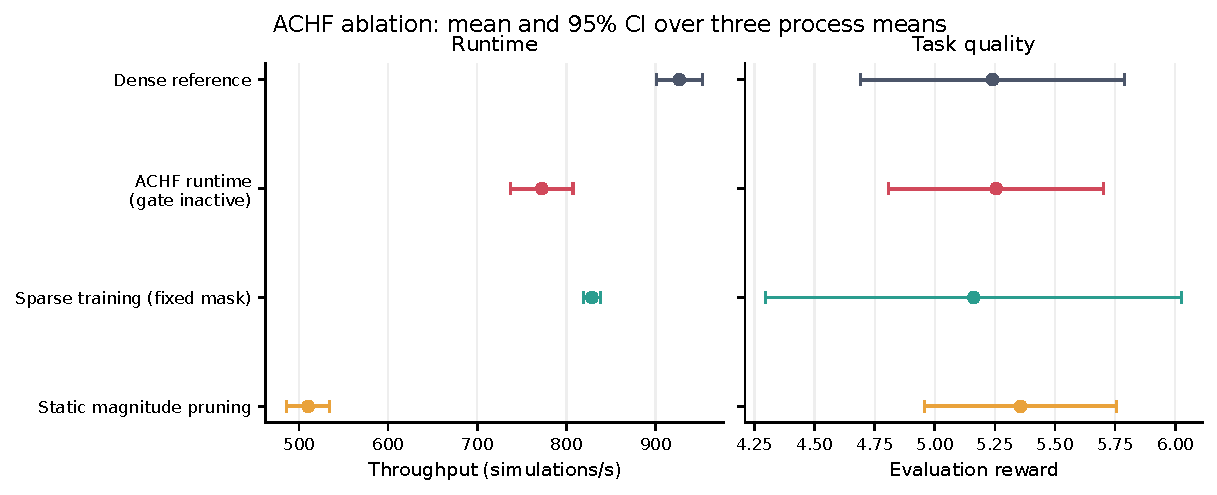
\includegraphics[width=\linewidth]{ablation_aggregate.pdf}
\caption{End-to-end ablation. Error bars are 95\% Student-$t$ intervals over
three independent process means.}
\label{fig:ablation-aggregate}
\end{figure}

The paired process-level throughput change for the ACHF runtime instantiation
relative to dense is
$-16.62\%$ (95\% CI $[-18.05,-15.19]\%$). Its training-time delta is
$+14.225$ s ($[12.463,15.988]$ s). Reward changes by $+0.0145$
($[-0.8043,0.8333]$) and loss by $+0.0429$ ($[-0.2424,0.3282]$), so neither
quality metric supports an improvement or an equivalence claim. Fixed-mask
sparse training is also slower than dense by $10.56\%$
($[-12.62,-8.50]\%$), while static magnitude pruning is slower by $44.93\%$
($[-47.14,-42.71]\%$). The current implementation therefore shows neither a
quality advantage nor a general end-to-end efficiency advantage.

\subsection{Fixed and Adaptive Execution Modes}

The mode experiment reuses the same trained policy across execution modes, so
reward, loss, and training time are identical by construction. It isolates
runtime routing. Table~\ref{tab:mode-results} shows that a fixed Prepared
Candidate is fastest on this stationary admitted workload. Guarded \ama{} is
faster than the plain EMA selector in mean throughput, but neither adaptive
selector reaches the known fixed winner.

\begin{table}[t]
\centering
\caption{Execution-mode throughput, mean [95\% CI] over process means. Paired
deltas are relative to Fixed Prepared Candidate. The raw benchmark label
\texttt{Cached} denotes this prepared-dense layout, not output memoization.}
\label{tab:mode-results}
\small
\begin{tabular}{lcc}
\toprule
Mode & Throughput (sim/s) & Paired delta \\
\midrule
Fixed Prepared Candidate & $899.51\ [890.84,908.17]$ & -- \\
Fixed Candidate Dense & $793.92\ [777.84,810.00]$ & $-11.73\%$ \\
Fixed Candidate CSR & $497.04\ [484.08,510.00]$ & $-44.75\%$ \\
Guarded \ama{} & $776.20\ [767.32,785.09]$ & $-13.70\%$ \\
Plain EMA & $742.04\ [730.37,753.71]$ & $-17.50\%$ \\
\bottomrule
\end{tabular}
\end{table}

The guarded/plain comparison supports a controller benefit over the simpler
online baseline, not a claim that online selection is free. In a stationary
regime where the best path is already known, fixed Prepared Candidate execution
remains the appropriate choice.

\subsection{Rank and Placement Sensitivity}

Every tested low-rank setting reduced throughput relative to no ACHF. Paired
process-level changes were $-7.54\%$ for rank 8, $-6.79\%$ for rank 16,
$-6.46\%$ for rank 32, $-7.15\%$ for rank 48, and $-6.23\%$ for the rank-64
no-op control; every 95\% interval remained below zero. No rank produced a
resolved reward or loss change. The no-op control has zero approximation error
but retains the slowdown, which identifies fixed ACHF bookkeeping and dispatch
as a material cost on this compact model rather than attributing all overhead
to approximation rank.

Placement results are similarly mixed. Table~\ref{tab:placement-results}
reports paired process-level contrasts against the corresponding no-ACHF PPO or
DQN reference.

\begin{table}[t]
\centering
\caption{Placement sensitivity. Values are paired mean [95\% CI]; training-time
deltas are seconds.}
\label{tab:placement-results}
\small
\resizebox{\linewidth}{!}{%
\begin{tabular}{lccc}
\toprule
Placement & Throughput delta & Reward delta & Train-time delta \\
\midrule
PPO Attention & $-6.48\%\ [-8.08,-4.88]$ & $-0.1523\ [-0.2641,-0.0405]$ & $+8.994\ [8.816,9.171]$ \\
PPO FFN & $+2.66\%\ [-0.17,5.48]$ & $+0.0174\ [-0.5787,0.6135]$ & $+11.108\ [7.279,14.937]$ \\
PPO FFN+Attention & $-3.71\%\ [-5.79,-1.63]$ & $+0.0415\ [-0.5713,0.6543]$ & $+14.895\ [13.022,16.767]$ \\
DQN hidden layer & $-16.94\%\ [-21.20,-12.69]$ & $+0.0948\ [-0.0973,0.2870]$ & $+0.208\ [0.176,0.241]$ \\
\bottomrule
\end{tabular}%
}
\end{table}

Attention-only placement is the one tested configuration with a resolved
reward regression as well as a throughput regression. FFN-only placement is
the only placement whose throughput point estimate is positive, but its
interval crosses zero and its training cost rises substantially. Thus FFN is a
reasonable target for further work, not a demonstrated improvement. The data
do not support enabling ACHF indiscriminately across attention and policy-head
layers.

\subsection{Convergence and Training Cost}

The longer convergence run gives the same direction as the main ablation.
ACHF-disabled throughput is $923.39\ [904.13,942.64]$ sim/s and enabled
throughput is $888.52\ [872.73,904.32]$ sim/s. The paired change is
$-3.76\%\ [-5.96,-1.56]\%$. Reward changes by
$-0.0629\ [-0.6089,0.4830]$, loss by
$+0.0419\ [-0.3380,0.4219]$, and training time by
$+15.084\ [13.425,16.743]$ s. This experiment supplies no evidence of faster
convergence or better final quality; it confirms a measurable training and
inference cost in the current implementation.

\subsection{Gate, Projection, and Optimizer Diagnostics}

The gate trace must be interpreted conservatively. Across all 16 recorded
training points in every process, the reference gate remained exactly $1.0$,
gate velocity remained zero, candidate eligibility was zero, and no candidate
output-discrepancy samples were recorded. The floor rose to $0.199764$ by step
4000, but the candidate did not enter the training blend. Consequently, this
run does \emph{not} empirically validate learned candidate-specific gate
dynamics. It validates reference anchoring during training; candidate quality
is evaluated separately during post-training calibration and admission.

The invariants that were exercised remained consistent. Sinkhorn normalization
was applied only to the dedicated nonnegative connection matrix, never to the
signed operator weight. At the final training point, maximum row and column
deviations were both $1.49\times10^{-8}$ in all process means, the negative
ratio was zero, the minimum entry was $0.01948$, and normalization used eight
iterations. After sparse projection and calibration, the maximum absolute
masked weight, masked gradient, and masked Adam moment were all zero in the
reported diagnostics. These observations support projection and optimizer-mask
consistency, but they are not a substitute for an experiment in which the
candidate gate actually moves. Because the candidate coefficient
$a=(1-g)\rho$ is zero when $g=1$, and frozen hard inference does not use this
soft blend, the run verifies the scaling invariant but does not measure a
quality or runtime benefit from the projected connection coordinate.

After freeze and admission, the gate experiment selected the candidate for
inference and routed $93.2$--$94.3\%$ of candidate calls through Prepared
Candidate, $0.9$--$1.0\%$ through Candidate CSR, and $4.7$--$5.9\%$ through
Candidate Dense. Mean selector
decision time ranged from $236.1$ to $263.4$ ns across processes. The quality
decision (reference versus candidate) and execution decision (Prepared
Candidate, Candidate CSR, or Candidate Dense realization) are therefore
reported separately. Raw artifacts retain the legacy path labels
\texttt{Cached}, \texttt{Sparse}, and \texttt{Dense}.

\subsection{Inference Materialization Cost}

The ACHF-enabled condition materializes multiple equivalent candidate layouts
simultaneously. This accounting covers runtime tensors for the four instrumented
ACHF layers only; it excludes the rest of the model, KV caches, allocator
overhead, and process RSS. Across all trials, these four reference layers used
98,816 bytes of reference parameters, while total materialized inference state
was 418,464 bytes, an additional 319,648 bytes and a
$4.23478\times$ ratio relative to reference-parameter storage.

\begin{table}[t]
\centering
\caption{Materialized inference memory for the evaluated ACHF runtime
instantiation. Counts are identical across all 15 trials; memoization is
disabled.}
\label{tab:memory-cost}
\small
\begin{tabular}{lr}
\toprule
Component & Bytes \\
\midrule
Reference parameters & 98,816 \\
Dedicated connection parameters & 64 \\
Candidate dense weights & 98,304 \\
Prepared Candidate weights and bias & 98,816 \\
Candidate CSR values, columns, and row pointers & 97,888 \\
Sparse mask & 24,576 \\
Memoized input and output & 0 \\
\midrule
Total materialized & 418,464 \\
\bottomrule
\end{tabular}
\end{table}

This accounting is a negative systems cost, not merely an implementation
detail. It motivates lazy layout construction, eviction, and a memory term in
future economic guards; none is implemented or evaluated here.

\subsection{Admitted Fixed-path Latency}

At the admitted $0.510010$ sparsity point, with input dimension 128, Prepared
Candidate is the fastest candidate realization by a wide margin
(Table~\ref{tab:path-latency-results}). Sparse traversal is approximately
$6.1\times$ slower than Prepared Candidate and $2.7\times$ slower than
Candidate Dense at this point.
This directly rejects any policy that equates successful sparsification with
permission to force sparse execution.

\begin{table}[t]
\centering
\caption{Fixed candidate-path latency at admitted $51.001\%$ sparsity, mean
[95\% CI] over process means.}
\label{tab:path-latency-results}
\small
\begin{tabular}{lc}
\toprule
Path & Latency (ns) \\
\midrule
Prepared Candidate & $456.9\ [439.6,474.3]$ \\
Candidate Dense & $1022.0\ [967.5,1076.4]$ \\
Candidate CSR & $2784.4\ [2714.8,2854.0]$ \\
\bottomrule
\end{tabular}
\end{table}

\subsection{Path Crossover}
\label{sec:crossover-results}

The admitted operating point does not favor sparse traversal, but sparse
execution can win when enough weights are removed.
Figure~\ref{fig:crossover-aggregate} measures the same candidate through
Prepared Candidate, Candidate CSR, and Candidate Dense realizations over three
matrix dimensions and five sparsity levels.

\begin{figure}[t]
\centering
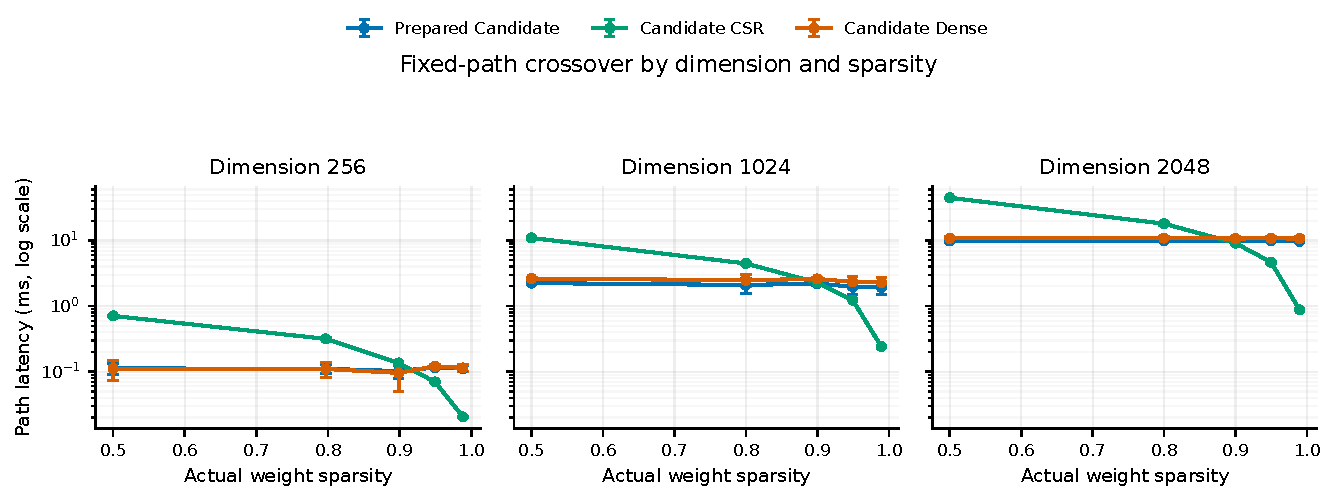
\includegraphics[width=\linewidth]{crossover_aggregate.pdf}
\caption{Fixed-path latency by dimension and actual weight sparsity. Points are
means and error bars are 95\% intervals over three process means. The vertical
axis is logarithmic.}
\label{fig:crossover-aggregate}
\end{figure}

Table~\ref{tab:crossover-winners} calls a path nominally supported only when
its paired 95\% difference interval is below both alternatives. These are
exploratory pointwise intervals with no multiplicity correction. At dimension
256, the small low-sparsity differences between Prepared Candidate and
Candidate Dense are unresolved. At dimensions 1024 and 2048, Prepared Candidate
wins at $0.50$ and $0.80$. Candidate CSR wins at $0.95$ and $0.99$ for every
tested dimension. Around $0.90$, the point winner varies with dimension and no
path has nominal paired support against both alternatives.

\begin{table}[t]
\centering
\caption{Nominally supported fixed-path regions without multiplicity
correction. Sparsity labels are the nominal grid points; the plotted values use
measured actual sparsity.}
\label{tab:crossover-winners}
\small
\begin{tabular}{lccc}
\toprule
Dimension & Supported Prepared Candidate & Unresolved transition & Supported Candidate CSR \\
\midrule
256 & -- & $0.50,0.80,0.90$ & $0.95,0.99$ \\
1024 & $0.50,0.80$ & $0.90$ & $0.95,0.99$ \\
2048 & $0.50,0.80$ & $0.90$ & $0.95,0.99$ \\
\bottomrule
\end{tabular}
\end{table}

For scale, at dimension 1024 and sparsity $0.50$, the means are 2.244 ms
(Prepared Candidate), 10.938 ms (Candidate CSR), and 2.634 ms (Candidate
Dense). At sparsity $0.99$, they are 1.931, 0.242, and 2.285 ms,
respectively. The data support a conditional crossover between $0.90$ and
$0.95$ on this machine, not a universal exact threshold.

\subsection{Steady-State Operating-Point Comparison}

This grid compares online selector latency with a hindsight oracle that chooses
the fastest fixed path for each sparsity and batch. Each point is warmed
independently before measurement; there is no within-run sparsity or batch
transition. It is therefore a steady-state operating-point comparison, not a
regime-transition or nonstationary-adaptation experiment. An oracle gap of $1$
is ideal. Table~\ref{tab:regime-results} and
Figure~\ref{fig:regime-aggregate} compare guarded \ama{} with a plain EMA
selector.

\begin{table}[t]
\centering
\caption{Selector/oracle latency ratio and paired difference, mean [95\% CI]
over process means. The last column is Guarded minus Plain; intervals are
nominal and are not multiplicity-corrected.}
\label{tab:regime-results}
\small
\resizebox{\linewidth}{!}{%
\begin{tabular}{ccccc}
\toprule
Sparsity & Batch & Guarded \ama{} & Plain EMA & Paired difference \\
\midrule
$0.80$ & 1 & $1.085\ [1.053,1.118]$ & $1.421\ [1.377,1.466]$ & $-0.3358\ [-0.4129,-0.2587]$ \\
$0.80$ & 128 & $1.096\ [1.067,1.125]$ & $1.154\ [1.070,1.237]$ & $-0.0575\ [-0.1120,-0.0030]$ \\
$0.90$ & 1 & $1.198\ [1.117,1.279]$ & $1.426\ [1.329,1.522]$ & $-0.2281\ [-0.2481,-0.2081]$ \\
$0.90$ & 128 & $1.047\ [1.015,1.079]$ & $1.026\ [1.022,1.031]$ & $+0.0205\ [-0.0136,+0.0547]$ \\
$0.95$ & 1 & $1.209\ [1.171,1.247]$ & $1.826\ [1.751,1.902]$ & $-0.6173\ [-0.7195,-0.5151]$ \\
$0.95$ & 128 & $1.095\ [1.075,1.115]$ & $1.152\ [1.004,1.300]$ & $-0.0572\ [-0.1858,+0.0713]$ \\
$0.98$ & 1 & $1.309\ [1.249,1.369]$ & $3.682\ [3.432,3.932]$ & $-2.3731\ [-2.5715,-2.1747]$ \\
$0.98$ & 128 & $1.179\ [1.164,1.193]$ & $1.859\ [1.717,2.000]$ & $-0.6799\ [-0.8096,-0.5502]$ \\
\bottomrule
\end{tabular}%
}
\end{table}

\begin{figure}[t]
\centering
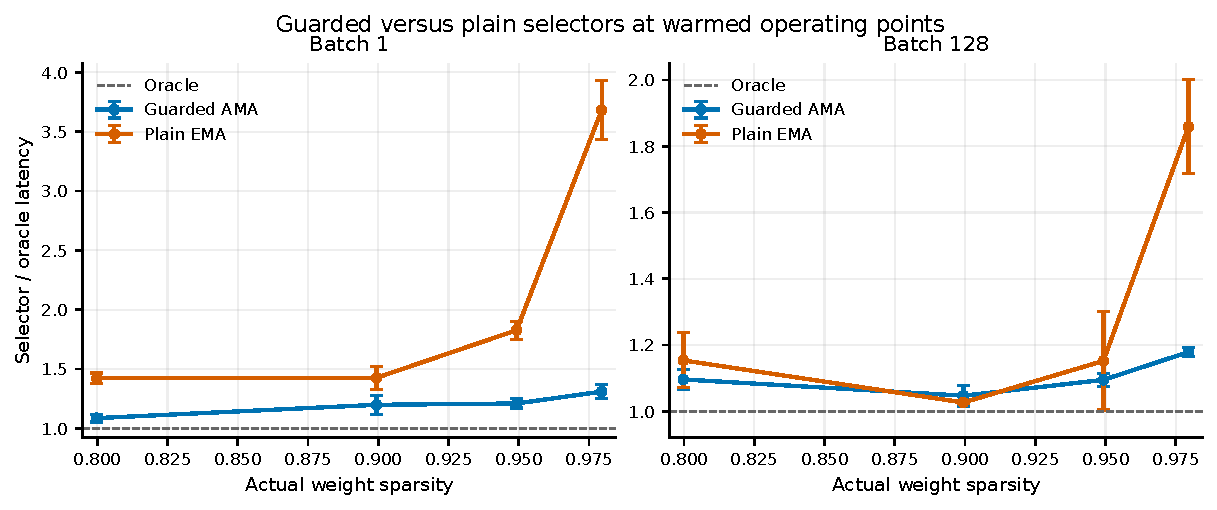
\includegraphics[width=\linewidth]{regime_aggregate.pdf}
\caption{Guarded and plain online-selector latency relative to the fixed-path
oracle. Lower is better; the dashed line is the oracle.}
\label{fig:regime-aggregate}
\end{figure}

Guarded \ama{} has the lower mean gap at seven of eight points. Six paired
intervals lie below zero; the $0.90$/batch-128 and $0.95$/batch-128 contrasts
are unresolved. At $0.90$/batch 128, Plain EMA has the lower mean. Every
guarded marginal interval remains above one, so guard overhead is measurable.
Together with Table~\ref{tab:mode-results}, the supported interpretation is a
guarded-versus-plain difference on this independently warmed grid. It does not
establish recovery, regret, or stability during an operating-point transition,
and a known fixed winner remains preferable in a stationary deployment.

An earlier single-invocation draft attributed a batch-driven oracle-path flip
to sparsity $0.90$. The replicated run does not reproduce that claim. The
process-level majority oracle is Prepared Candidate for both batch sizes in all
three processes (two batch-1 processes contain one Candidate CSR trial, but
Prepared Candidate remains the majority). We therefore remove the batch-flip
claim rather than preserving the old favorable narrative.

\subsection{Answers to the Evaluation Questions}

\textbf{RQ1, task quality.} No measured ACHF condition establishes a general
reward or loss improvement. Attention-only placement has a resolved reward
regression. The remaining quality intervals are unresolved.

\textbf{RQ2, runtime behavior.} The current end-to-end implementation is slower
than dense. Path-level evidence is conditional: Prepared Candidate wins at the
admitted $51\%$ point, while Candidate CSR wins only at high sparsity in the
tested grid. Guarded ranking has lower mean oracle gap than Plain EMA at seven
of eight independently warmed points, with six nominal paired intervals below
zero, but does not beat a known fixed winner.

\textbf{RQ3, measured invariants.} Dedicated connection scaling and sparse
weight/gradient/optimizer masks satisfy their measured invariants. The training
run does not exercise adaptive candidate gating, so no gate-adaptation
stability claim follows from it, and projection utility remains unmeasured.

\textbf{RQ4, evaluated component evidence.} Configured admission excludes
candidates outside its predicate, and guarded ranking has a lower mean gap than
Plain EMA at seven of eight grid points. Rank controls and broad placement do
not recover the fixed overhead; FFN-only placement is the only nonnegative
throughput point estimate, and that estimate remains unresolved. The run does
not isolate projection utility, active-gate value, a complete economic bypass,
or exact-reuse value.

\section{Discussion}

The results materially narrow the design claim. Candidate admission works as a
quality boundary, but candidate admission and execution-path selection cannot
be collapsed into one decision: the admitted $51\%$ sparse candidate is best
executed through its Prepared Candidate realization, not through Candidate CSR.
Conversely, Candidate CSR becomes useful at sufficiently high sparsity, even
though those more aggressive candidates fail the present task-quality
admission threshold. This is precisely why ACHF keeps a quality decision, an
execution decision, and an exact memoization fast path as separate layers.

The measurements also expose costs that the formulation alone cannot remove.
The ACHF runtime instantiation loses end-to-end throughput, the rank-64 no-op
control remains slower, materialized ACHF-layer state is $4.235\times$ its
reference-parameter bytes, and guarded selection retains a positive oracle
gap. Guarding is useful here only as a measured improvement over a weaker
online selector at most steady-state grid points, not as a replacement for a
known fixed path or as evidence of transition recovery. Finally, the unchanged
training gate means this case study does not test the most ambitious
adaptive-gating part of the method. These are implementation and evidence
limits, not numbers to be explained away as automatic tradeoffs.

\achf{} is best understood as a runtime-coupled architectural idea. The point
is not to claim pruning, projection, or caching as separate inventions. The
point is to keep them in the same connection lifecycle. Projection constrains the
connection map when such a constraint has a clear interpretation. Gating keeps
a stable reference path available during training, but the gate must be tied to
candidate quality rather than to gradient statistics alone. Candidate
construction creates an alternative execution form. The runtime then chooses
among available paths using measured behavior, including whether a path is cold
or warmed.

\ama{} is the separable control algorithm for this lifecycle. It does not
define what the candidate path is, nor does it require the candidate to come
from ACHF. It defines when a candidate can be trusted: validity first, then
positive measured economics, stale-path refresh, switch hysteresis, and
optimizer-state observability. The additional cold/warm latency state and
candidate-discrepancy signal are included because the simpler design is too
easy to fool: a smooth gradient does not prove a candidate is accurate, and a
single cold probe does not prove a path is slow. In this sense, ACHF describes a
class of adaptive connection layers, while \ama{} describes a guarded way to
operate any reference/candidate execution system.

This differs from conventional pruning, where the pruned network is usually
treated as the final model. \achf{} keeps a reference path in the model
lifecycle and uses it as a stability anchor. It also differs from a full
manifold-constrained Hyper-Connection architecture: the case-study
implementation does not implement separate dynamic $H_{\mathrm{pre}}$,
$H_{\mathrm{post}}$, and $H_{\mathrm{res}}$ maps. Instead, it adapts the
constrained-connection principle to a practical dense/candidate operator blend.

\section{Threats to Validity}

\textbf{Statistical validity.}
The independent unit is a process mean and $N=3$, leaving two degrees of
freedom. The five trials per process improve each process estimate but do not
increase the independent-process sample size. Intervals are therefore wide,
and the many diagnostic comparisons are exploratory rather than corrected for
family-wise testing. No interval crossing zero is interpreted as equivalence.

\textbf{Hardware and measurement validity.}
All processes ran sequentially on one CPU/software environment. Native CPU
code generation, operating-system scheduling, frequency scaling, and cache
state may affect absolute timings. Rotating interleaved condition order reduces
drift within each process, but it does not replace replication on another CPU,
operating system, or GPU. CUDA and BF16 execution are not evaluated here.

\textbf{Workload validity.}
Talos-XII is a custom Rust runtime with compact PPO and DQN policies. The
crossover and steady-state selector grids use controlled matrix
microbenchmarks, while the
task metrics come from a stochastic simulator. Neither directly establishes
behavior for large transformers, distributed training, standard benchmark
datasets, or mature sparse-library kernels.

\textbf{Runtime-control validity.}
The fixed-mode experiment gives the selector a stationary workload and shows
that Fixed Prepared Candidate is faster than both online selectors. Every point
in the selector grid is independently warmed. The experiment therefore shows a
guarded/plain difference only at steady-state operating points; it measures no
transition recovery, cumulative regret, or nonstationary interference.

\textbf{Calibration validity.}
Calibration uses an index-modulo-four 75/25 split of temporally adjacent rollout
states. Context windows may overlap, and the validation subset is used for both
early stopping and final admission. The resulting $0.51$ choice is also selected
after inspecting the same exploratory frontier. A stronger evaluation requires
episode- or seed-separated calibration, tuning, and final-admission sets.

\textbf{Gate-signal validity.}
The candidate gate does not move in this run and candidate discrepancy is not
sampled during training. Post-training calibration demonstrates candidate
admission, not candidate-aware training. Claims about learned gate adaptation,
gradient-only versus discrepancy-aware gating, or gate-induced optimizer drift
require a run in which candidates actually participate in the training blend.

\textbf{Projection and optimizer validity.}
The dedicated connection matrix satisfies its measured Sinkhorn constraints,
and masked weights, gradients, and Adam moments are zero after calibration.
These endpoint invariants do not prove long-horizon optimization stability.
They also do not establish projection utility: in the one-candidate blend,
$g$ and $\rho$ enter only through $(1-g)\rho$, the measured gate stays at one,
and hard inference bypasses the soft coefficient. Nor do the invariants justify
applying Sinkhorn to arbitrary signed operator weights; the case study
deliberately does not do so.

\textbf{Baseline and external validity.}
The suite includes dense, static magnitude, fixed-mask sparse-training,
fixed-path, Plain EMA, no-op rank, and placement controls. It does not include
an optimized external sparse library, a non-ACHF \ama{} system, early exit,
MoE routing, or a matched implementation in a standard framework. General
method superiority and transfer beyond this one task/runtime therefore remain
unmeasured.

\section{Limitations}

\begin{itemize}[leftmargin=*]
\item The ACHF runtime instantiation with inactive training gate is slower than
the dense reference in both main and convergence experiments, takes longer to
train, and has no resolved reward or loss benefit.
\item All aggregate intervals contain only three independent process means and
all processes use one CPU/software environment.
\item The training trace remains on the reference gate; learned adaptive gating
and candidate-aware optimizer dynamics are not empirically exercised.
\item The $51\%$ point is a same-frontier exploratory selection, not an
independently validated operating point; calibration uses overlapping temporal
contexts and one validation subset for early stopping and final admission.
\item At the admitted $51\%$ sparsity point, Candidate CSR is the slowest
realization. The points where it wins the microbenchmark are too inaccurate to
pass the current task-level admission criteria.
\item Guarded \ama{} has lower mean oracle gap than Plain EMA at seven of eight
independently warmed points, but two paired contrasts are unresolved, all
guarded gaps remain above one, and Fixed Prepared Candidate wins the stationary
mode experiment. No transition experiment was run.
\item Materialized runtime tensors for the four ACHF layers occupy 418,464
bytes versus 98,816 reference-parameter bytes ($4.23478\times$). This is not
whole-model memory or process RSS, and no lazy-layout or eviction policy is
evaluated.
\item The evaluated selector does not instantiate the proposed complete
baseline-relative economic bypass; exact-output memoization is disabled and
has no speedup evidence.
\item FFN-only placement has a positive throughput point estimate but an
interval crossing zero and a large training-time cost; attention placement
reduces measured reward.
\item CUDA, BF16, other CPUs, standard ML frameworks, larger architectures, and
external sparse libraries are not evaluated.
\item Several method-level comparison targets remain absent, including a
non-ACHF \ama{} system and matched early-exit or MoE routing baselines.
\item Sinkhorn scaling invariants are checked only for dedicated nonnegative
connection matrices, not signed operator weights; its component utility is not
isolated.
\item The case study does not implement the full dynamic mHC formulation;
\achf{} is a related but distinct design that adapts constrained
hyper-connection ideas toward runtime-adaptive execution.
\end{itemize}

\section{Conclusion}

\achf{} formulates runtime-adaptive neural connections as three explicit
layers: reference/candidate quality selection, execution-path selection for an
admitted candidate, and exact memoized reuse. A dedicated connection matrix may
be projected when its semantics justify the constraint, while operator weights
and optimizer state follow their own sparse mask. \ama{} supplies guarded
measurement, probing, and switching for the execution layer.

The completed Talos-XII case study supports only part of that proposal. The
configured admission predicate has one fully admitted tested frontier point,
connection-scaling and mask invariants hold, fixed-path winners change with
sparsity, and guarded \ama{} has lower mean oracle gap at seven of eight
independently warmed grid points, with six nominal paired intervals below zero.
At the same time, the ACHF runtime instantiation is $16.62\%$ slower than dense
in the main ablation, adds 14.225 s of training, materializes
$4.23478\times$ the ACHF-layer reference-parameter bytes, does not improve
reward or loss, and never activates the candidate gate during training.
Prepared Candidate rather than Candidate CSR is fastest at the admitted point.
These results make ACHF a conditional runtime design with an explicit negative
case study, not a demonstration of universal neural quality or efficiency.
Cross-hardware replication, separate final admission data, a true transition
test, and an experiment that genuinely exercises adaptive gating are the next
empirical requirements.

\section*{Reproducibility Checklist}

\begin{itemize}[leftmargin=*]
\item Public source: \url{https://github.com/zayokami/Talos-XII}
\item ACHF implementation: \texttt{src/achf.rs}; benchmark implementation:
\texttt{src/bench.rs}.
\item Completed full-run command:
\begin{verbatim}
cargo run --release -- benchmark paper --trials 5 --processes 3 `
  --format svg --output-dir target/release/bench_output_final
\end{verbatim}
\item Statistical unit: independent process mean, $N=3$; five paired trials per
process; two-sided Student-$t$ 95\% intervals with two degrees of freedom.
\item Integrity: all three process manifests are complete; 30 artifacts per
process and all 90 hashes are verified by the parent manifest.
\item Environment: Intel Core i9-13900HX, 32 logical processors, 31.8 GiB RAM,
Windows build 26200.8875, Rust/Cargo 1.93.1, release CPU build, CUDA disabled.
\item Cache policy: existing executable-adjacent caches were recorded but
ignored; benchmark models were rebuilt from domain-separated seeds.
\item Raw artifact: immutable public archive URL pending upload and required
before submission. The local verification directory
\texttt{target/release/bench\_output\_final} is not a public artifact.
Aggregate figure script: \texttt{docs/plot\_aggregate\_results.py}; generated
figure data: \texttt{docs/media/aggregate\_figure\_data.json}.
\item Outstanding external replication: a second hardware/software environment
and a training configuration in which the candidate gate actually participates.
\end{itemize}

\bibliographystyle{unsrt}
\bibliography{references}

\end{document}